%====================================================
%	CHAPTER 6 - Control & Simulations
%====================================================
\chapter{Simulations and Results}
\label{ch:simulation}
%====================================================
\section{Simulator description}
\label{sec:simulation.block}
%====================================================
The proposed attitude and position control laws, together with the system dynamic equations of motion including each actuator's transfer function, were all tested in simulation to determine a particular controller's efficacy. The rigid-body equations of motion from Sec:\ref{subsec:dynamics.rigidbody.lagrange}, with non-linearities from Sec:\ref{sec:dynamics.aero} and multi-body responses from Sec:\ref{sec:dynamics.nonlinearities}, were incorporated into a high fidelity simulation environment. Closely matching the dynamics of the physical quadrotor prototype proposed in Sec:\ref{sec:proto.design}; using measurement data produced by tests in Sec:\ref{subsec:dynamics.nonlinearities.torque-tests} to provide a degree of confidence in the simulation's accuracy. The consolidated quaternion dynamics in Sec:\ref{sec:dynamics.model} formed the basis of the simulation; building a loop extended from the control structure in Fig:\ref{fig:control-block}. Each control law is optimized first without the effect of the servo's $180$\textdegree ~saturation limit. Limiting the servos was a conscientious design decision and as such its effects are investigated in Sec:\ref{sec:simulation.saturation}; but for now the servos are treated as continuous\ldots
\par
\begin{figure}[htbp]
\vspace{-10pt}
\centering
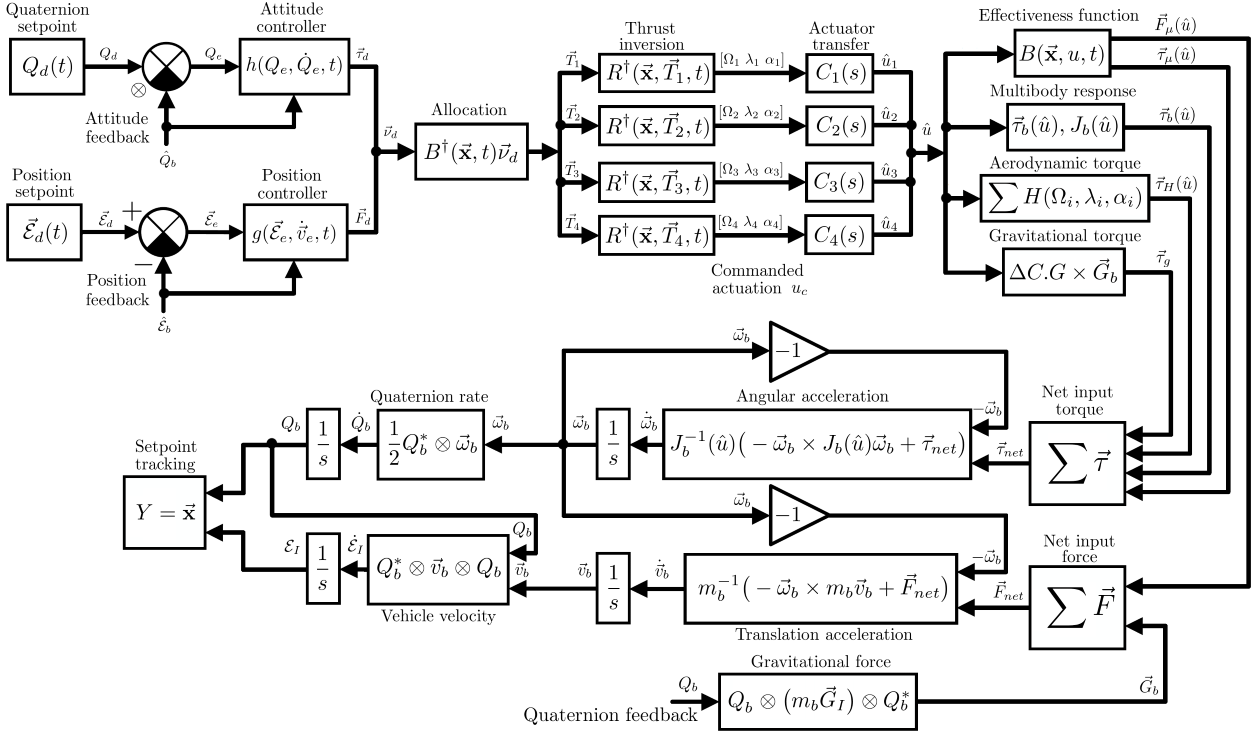
\includegraphics[width=0.93\textwidth]{figs/simulation-block}
\vspace{-10pt}
\caption{Simulation loop}
\label{fig:simulation-block}
\end{figure}
\vspace{-12pt}
\par
An abstracted simulation loop is illustrated in Fig:\ref{fig:simulation-block}; incorporating both attitude and position control loops together with the additive non-linearities. Certain feedback elements were omitted to retain clarity in the diagram, both Coriolis and Gyroscopic non-linear couplings were included. Not shown is some form of state-estimation discretization between the state-tracking output $y=\vec{\mathbf{x}}=[Q_b,~\vec{\mathcal{E}}\hspace{2pt}]^T$ and the feedback state $\hat{\mathbf{x}}$ used for setpoint tracking. Discretized effects of state-estimators are discussed later in Sec:\ref{sec:simulation.state}.
\par
Initial conditions for each state integrator, both position and attitude accelerations $\dot{\vec{v}}_b$ and $\dot{\vec{\omega}}_b$, and their velocities $\dot{\mathcal{E}}_b$ and $\dot{Q}_b$ respectively, are not illustrated but implied. Obviously starting conditions are important for each trajectory's simulation but are specifically defined for each simulation in question. Actuator transfer functions from Sec:\ref{subsec:proto.design.transfer} are combined into a bundled $H_{i}(S)$ block, accounting for transfer functions and the saturation limits of each motor module. Each bundled input $u_{1\rightarrow 4}$ is similarly the projected actuator matrix:
\begin{equation}
u_{i}=u\cdot i = \begin{bmatrix}
\Omega_i & \lambda_i & \alpha_i
\end{bmatrix}~~~~\text{for}~i\in[1:4]
\end{equation}
Then $\vec{T}_i(S)$ is the resultant thrust vector from a single motor module with a combined MIMO transfer function. Lastly the setpoints for both attitude and position states are either stepped set points or produced from a simple orbital trajectory. The former is used for controller optimization and the latter is used to evaluate each controller's setpoint tracking performance. To discuss the question of non-zero setpoint tracking an orbital trajectory is generated; shown in Fig:\ref{fig:trajectory}.
\begin{figure}[htbp]
\centering
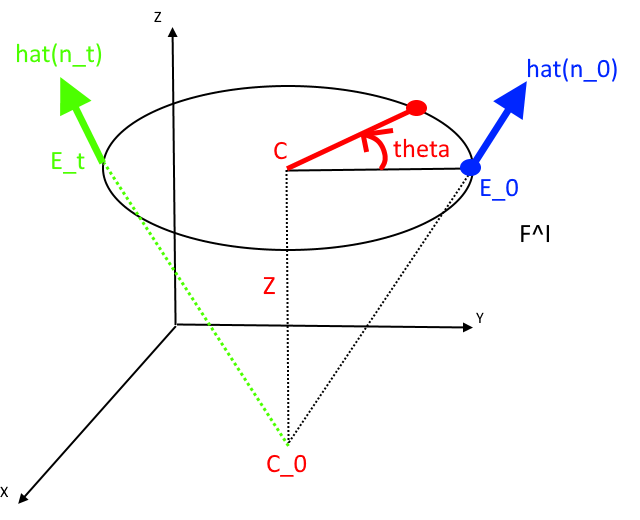
\includegraphics[width=0.5\textwidth]{figs/trajectory}
\caption{Orbital trajectory}
\label{fig:trajectory}
\vspace{-18pt}
\end{figure}
\par
The trajectory generates only attitude and position setpoints; a trajectory is entirely independent from actuator values for the aircraft's configuration. For a central point in the inertial frame $\vec{C}_0\in\mathcal{F}^I$, the trajectory orbits at an angular rate of $\dot{\theta}~[\text{Hz}]$ around that center. The orbit is at a height of $\hat{z}_c~[\text{m}]$ and at a radius $R_c~[\text{m}]$ from the center $\vec{C}$. The position setpoint then follows:
\begin{subequations}
\begin{equation}
\vec{\mathcal{E}}_{d}(t)=\begin{bmatrix}
C_{0x}+R_c\cos \theta(t)\\
C_{0y}+R_c\sin \theta(t)\\
\hat{z}_c
\end{bmatrix}~~~~\in\mathcal{F}^I
\end{equation}
The time varying trajectory's attitude setpoint is aligned with a normal vector $\hat{n}_d(t)$, pointing away from the center point $\vec{C}_0$:
\begin{equation}
\hat{n}_d(t)\triangleq\frac{\vec{\mathcal{E}}_d(t)-\vec{C}_0}{\sqrt{\hat{z}_c^2+R_c^2}}
\end{equation}
The quaternion setpoint is then constructed from $\hat{n}_d$ such that:
\begin{equation}
Q_d(t)=\begin{bmatrix}
\sin \frac{\theta(t)}{2} & \cos \frac{\theta(t)}{2}\hat{n}_d(t)
\end{bmatrix}^T
\end{equation}
\end{subequations}
Neither first order nor higher derivative setpoints are applied for the trajectory in Fig:\ref{fig:trajectory}. Both position and attitude rates are respectively $\dot{\vec{\mathcal{E}}}_d(t)=\vec{0}$ and $\dot{Q}_d(t)=\vec{0}$ throughout the entire trajectory, as per Eq:\ref{eq:4.85a} and Eq:\ref{eq:4.27c}.
%====================================================
\section{Controller Tuning}
\label{sec:simulation.tuning}
%====================================================
Each controller's derivation and stability, shown previously in Ch:\ref{ch:control}, demonstrated only a control law's setpoint tracking ability; providing no further insight into the controller coefficient design. Lyapunov stability theorem, in the context of Sec:\ref{sec:control.attitude}-\ref{sec:control.position}, evaluates a particular trajectory's stability over $t\rightarrow\infty$ but nothing more. Often at the coefficient selection stage a \emph{monte carlo} approach is applied; in most cases choosing coefficients seemingly at random and haphazardly, without any obvious forethought or design\ldots 
%====================================================
\subsection{Partical Swarm Based Optimization}
\label{subsec:simulation.tuning.pso}
%====================================================
Particle swarm based optimization (\emph{PSO}) has been shown in both \cite{adaptivepso} and \cite{autopilotPSO}, amongst others, to be an effective controller coefficient design tool. The algorithm treats each variable to be optimized as a \emph{particle} which exists within some defined search space. The collection or \emph{swarm} of particles explores the search space directed by both the swarm's previous performance as well as the relative performance between each particle. In \cite{particletrajectories} the statistical nature of the swarm's trajectory is discussed, however such investigations are well beyond the scope of this work.
\par
In general the PSO algorithm applies a \emph{gradient free} based search of solutions for a given optimization problem. The lack of a specified gradient is an important distinction which differentiates PSO from other algorithms. Often a predefined gradient function is required to direct the optimization search; MatLab's own Fmincon\cite{fmincon} or Interior-Point optimizer\cite{ipopt} algorithms for example. Interval gradient calculations can be computationally exhaustive and reduce the rate of execution for the entire process. An optimizer's performance is directly proportional to the number of complete iterations it executes, if an iteration has a high degree of complexity (read \emph{stiffness}) it's solution time is then adversely effected. The PSO algorithm is defined as follows; if there exists a set $\vec{x}$ of $k$ variables, $\vec{x}\in\mathbb{R}^{k\times 1}$ to be optimized. The swarm of $\vec{x}_n$ particles, which starts at the position $\vec{x}_0$, has an $n^{\text{th}}$ interval which progresses through the search space as per the velocity function:
\begin{subequations}
\begin{equation}
\vec{x}_{n+1}=\vec{v}_{n}+x_{n}
\end{equation}
\vspace{-18pt}
\begin{equation}\label{eq:swarm-velocity}
\vec{v}_{n+1}\triangleq w\ast \vec{v}_n+c_1\ast r_1\big(\vec{P}_{best}-\vec{x}_n\big)+c_2\ast r_2\big(\vec{G}_{best}-\vec{x}_n\big)
\end{equation}
\end{subequations}
\par
\begin{figure}[hbtp]
\vspace{-20pt}
\centering
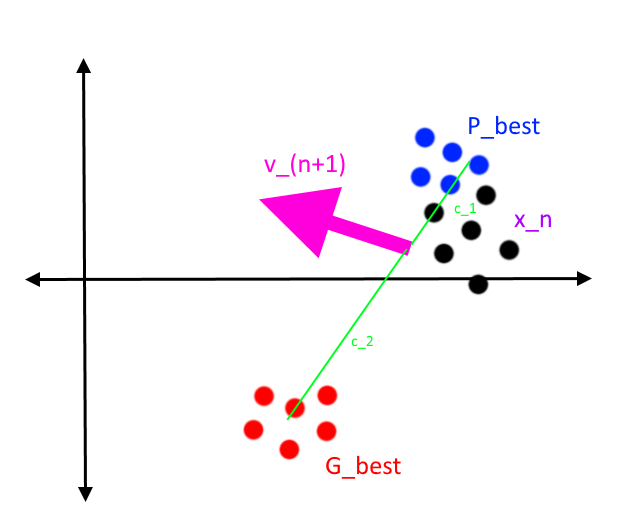
\includegraphics[width=0.54\textwidth]{figs/swarm-trajectory}
\vspace{-10pt}
\caption{Swarm trajectory's velocity direction}
\label{fig:swarm-trajectory}
\vspace{-18pt}
\end{figure}
\par
Each $\ast$ operator in Eq:\ref{eq:swarm-velocity} applies an element-by-element matrix coefficient multiplication. Both $\vec{P}_{best}$ and $\vec{G}_{best}$ are previous swarm positions where local and global optima were respectively achieved. Performance of the swarm's current interval is evaluated as per some cost function, responding to a system's dynamics; expanded on next. Finally $r_1$ and $r_2$ are random seeded $\mathbb{R}^{1\times k}$ exploratory matrices which progress the search direction, biased by the two weighting coefficients $c_1$ and $c_2$. The search is prejudiced toward local optima by $c_1$ whilst $c_2$ directs the swarm toward global optima. Fig:\ref{fig:swarm-trajectory} illustrates how positions of both local and global optima influence subsequent velocities.
\par
The swarm's interval performance is evaluated by the response of a dynamic system to the swarm's position;  typically an error deviation away from some desired state. Here, the simulation described in Fig:\ref{fig:simulation-block}, is parsed a swarm of controller coefficients as an argument and the plant's setpoint response is simulated over a series of step tests. Particulars with regards to attitude controller optimization is discussed in Sec:\ref{sec:simulation.attitude}, thereafter position controller optimization is detailed in Sec:\ref{sec:simulation.position}. The objective is for zero-error setpoint tracking so each swarm's coefficient performance metric calculates an integral-time-absolute-error (\emph{ITAE}) cost, \cite{ITAE}.
\begin{equation}
\vec{\zeta}\triangleq\int_{t_0}^{t_\infty}t|\vec{e}(t)|.dt
\end{equation}
With an error $\vec{e}(t)$ deviating from the plant's given setpoint. The ITAE integral is evaluated over the entire simulation time or an effective $t_\infty$. The time multiplier ensures setpoint error \emph{and} settling time optimality; punishing overshoot and under-damped or oscillatory like behaviour.
\par
In general a PSO algorithm follows the flow diagram in Fig:\ref{fig:particle-diagram}. Because each controller was empirically proven to be stable independent of it's trajectory; the controller will settle irrespective of the proposed interval coefficient values. A consequence of this is the starting conditions for the swarm, $\vec{x}_0$, have no bearing on the progression of the optimization. A round set of unity coefficients were selected as a starting point for each controller's optimization\ldots
\begin{figure}[htbp]
\centering
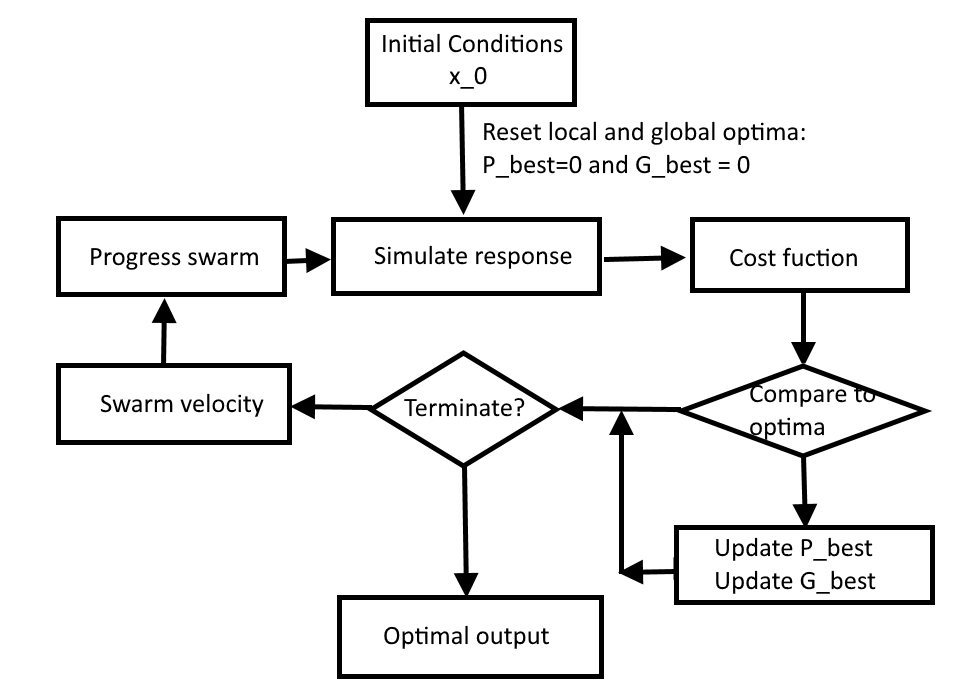
\includegraphics[width=0.7\textwidth]{figs/particle-diagram}\vspace{-12pt}
\caption{Particle swarm flow diagram}
\label{fig:particle-diagram}
\vspace{-18pt}
\end{figure}
\par
Termination conditions for the iterative optimization loop either limit the number of iteration cycles performed or break from the process once a result is regarded as sufficiently close to optimal. Each optimization cycle was iterated for $tx=1000$ times, testing and evaluating one thousand different swarm values for a series of stepped setpoints. As the optimizer progressed through iterations it adapted it's bias from a global to local optima, refining the way in which it searched for potential controller coefficients.
\begin{equation}
\vec{v}_{n+1}=\vec{v}_n+\frac{tx}{1000}\ast r_1(\vec{P}_{best}-\vec{x}_n)+\frac{1000-tx}{1000}\ast r_2(\vec{G}_{best}-\vec{x}_n)~~~~\text{for}~tx\in[1:1000]
\end{equation}
This gave each controller an equal likelihood of reaching optimality. Obviously controllers which improve their performance between each iteration at a faster rate were biased here. Moreover each swarm's progression was constrained such that it never violated the Lyapunov stability conditions of it's respective control law\ldots
%====================================================
\section{Attitude Controllers}
\label{sec:simulation.attitude}
%====================================================
Attitude controllers derived in Sec:\ref{sec:control.attitude} were optimized first, owing to their independence from the position loop. Constant hovering force condition was simply applied to the virtual plant input $\vec{F}_d$ for each test. A pseudo inversion allocator, Sec:\ref{subsec:allocation.allocators.inverse}, was applied to the control loop when testing each attitude controller. To evaluate an individual swarm's performance a number of step tests were performed. Each attitude setpoint was first defined in the Euler angle parametrization, being conceptually easier to visualize. Thereafter the attitude setpoints were converted into a quaternion attitude and applied to the simulation.
\begin{equation}
\vec{\eta}_d(t)\triangleq \begin{bmatrix}
\phi_d(t)&
\theta_d(t)&
\psi_d(t)
\end{bmatrix}^T\underset{Q}{\iff}Q_d(t)
\end{equation}
Each of the three Euler angles were stepped in the range $[-90\text{\textdegree}:+90\text{\textdegree}]$ at an interval of $30\text{\textdegree}$. This resulted in a test of 343 possible attitude setpoints; making a workspace sphere as illustrated in Fig:\ref{fig:attitude-setpoint}. Each attitude step was allowed $t=15~[\text{s}]$ to reach its settling point, with an initial attitude position always set to the origin $Q_b(t_0)=[1~\vec{0}\hspace{2pt}]$, with a \emph{positive} quaternion scalar. The performance for each attitude step test was evaluated by an ITAE integral for the quaternion error vector and angular velocity error:
\begin{equation}\label{eq:attitude-performance}
\vec{\zeta}_{Q}=C_Q\int_{t=0}^{15}t|\vec{q}_e(t)|.dt+C_\omega\int_{t=0}^{15}t|\vec{\omega}_e(t)|.dt~~~~\in\mathbb{R}^{3}
\end{equation}
Weighting coefficients $C_Q$ and $Q_\omega$ balance priority of either quaternion or angular velocity tracking, however, tracking both were equally important and so those weights were $C_Q=Q_\omega=1$. The cost integral in Eq:\ref{eq:attitude-performance} was averaged over all 343 possible attitude steps to ascertain the overall performance of a proposed swarm of coefficients.
\begin{figure}[htbp]
\centering
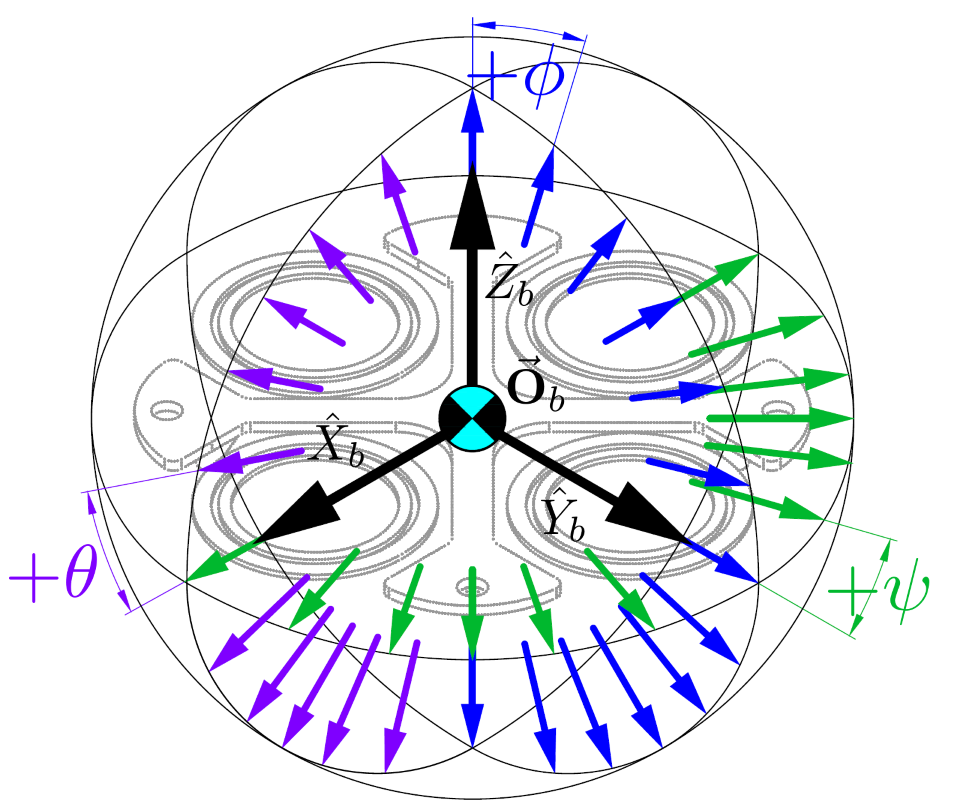
\includegraphics[width=0.65\textwidth]{figs/attitude-setpoint}
\caption{Attitude setpoint working space}
\label{fig:attitude-setpoint}
\end{figure}
\par
The integral in Eq:\ref{eq:attitude-performance} produces a vector $\in\mathbb{R}^{3}$ result. Each coefficient in a particular controller contributes towards a local error in one of the $\hat{X},\hat{Y},\hat{Z}$ components, or in certain cases a pair of axial components. Each controller's local errors and the coefficients which affect them are discussed subsequently. A global error for the performance of each controller is simply the magnitude $\norm{\vec{\zeta}_Q}$. The same global error is applicable to all controllers\ldots
\par
To compare the relative performance and effectiveness of each optimized control structure a single attitude step was investigated. That attitude change was chosen to be a sizeable step in all three Euler angles:
\begin{equation}\label{eq:attitude-step-position}
\vec{\eta}_d=\begin{bmatrix}
\phi_d\\
\theta_d\\
\psi_d\\
\end{bmatrix}
=
\begin{bmatrix*}[r]
-142\text{\textdegree}\\
167\text{\textdegree}\\
-45\text{\textdegree}
\end{bmatrix*}
\underset{Q}{\iff}
\begin{bmatrix}
-0.3254&
0.2226&
-0.2579&
0.8821
\end{bmatrix}^T
\end{equation}
Then each controller's settling time to $95$\% of it's final value, $t_{95}$, and it's relative angular velocity (the setpoint for which is $\vec{\omega}_d=\vec{0}$) for such a step is evaluated. Settling time, overshoot and setpoint error are all factors to consider when discussing a controller's efficacy. Lastly, commanded (virtual) and applied input torque to the actuator set are discussed too. A feasible controller should not induce torque saturation or unachievable input rate changes.
%====================================================
\subsection{PD}
\label{subsec:simulation.attitude.pd}
%====================================================
The first controller evaluated, the Proportional-Derivative structure, is investigated under three different circumstances. Before discussing each of those different scenarious, it is worth recalling that control structure from Sec:\ref{subsubsec:control.attitude.controllers.pd}. The control torque is designed by two coefficient matrices $K_p$ and $K_d$:
\begin{equation}\label{eq:simulation-attitde-pd}
\vec{\tau}_{_{PD}}=\underbrace{K_p\vec{q}_e+K_d\vec{\omega}_e}_{Independent}+\underbrace{\vec{\omega}_b\times J_b(u)\vec{\omega}_b+\hat{\tau}_b(u)-\vec{\tau}_g-\vec{\tau}_Q}_{Compensation}~~~~\in\mathcal{F}^{b}
\end{equation}
The first two tests regard both coefficient matrices as purely diagonal, with no skew elements; evaluating the effect inclusion of plant dependent compensation has on the controller's performance. Finally a plant dependent compensating PD controller is tested \emph{with} symmetrical coefficient matrices. The diagonal coefficient matrices are defined and numbered as follows:
\begin{equation}\label{eq:simulation-attitde-pd-diagonal-coefficients}
K_p\triangleq \begin{bmatrix}
K_p(1) & 0 & 0\\
0 & K_p(2) & 0\\
0 & 0 & K_p(3)
\end{bmatrix}
~~\text{and}~~K_d\triangleq \begin{bmatrix}
K_d(1) & 0 & 0\\
0 & K_d(2) & 0\\
0 & 0 & K_d(3)
\end{bmatrix}
\end{equation}
Then selection of each local and global position for the PSO algorithm needs to be defined. The proportional coefficient $K_p$ acts on $\vec{q}_e$ whilst the derivative coefficient $K_d$ acts on $\vec{\omega}_e$. Naturally the local and global optimal position are then selected and updated:
\begin{equation}
\vec{P}_{Best}\equiv
\begin{bmatrix}
K_p(1)\Rightarrow \min \vec{q}_e(1)\\
K_p(2)\Rightarrow \min \vec{q}_e(2)\\
K_p(3)\Rightarrow \min \vec{q}_e(3)\\
K_d(1)\Rightarrow \min \vec{\omega}_e(1)\\
K_d(2)\Rightarrow \min \vec{\omega}_e(2)\\
K_d(3)\Rightarrow \min \vec{\omega}_e(3)
\end{bmatrix}~~\text{and}~~\vec{G}_{Best}\equiv\begin{bmatrix}
K_p(1)\Rightarrow \min \vec{\zeta}_{_{PD}}(1)\\
K_p(2)\Rightarrow \min \vec{\zeta}_{_{PD}}(2)\\
K_p(3)\Rightarrow \min \vec{\zeta}_{_{PD}}(3)\\
K_d(1)\Rightarrow \min \vec{\zeta}_{_{PD}}(1)\\
K_d(2)\Rightarrow \min \vec{\zeta}_{_{PD}}(2)\\
K_d(3)\Rightarrow \min \vec{\zeta}_{_{PD}}(3)
\end{bmatrix}
\end{equation}
Where each local or global best coefficient position is updated if the minimum (best) result is improved on. For the symmetrical coefficient case, each off-diagonal element acts on two components of the error states. Those controller coefficients are then numbered:
\begin{equation}\label{eq:simulation-attitde-pd-symmetric-coefficients}
K_p\triangleq \begin{bmatrix}
K_p(1) & K_p(4) & K_p(5)\\
K_p(4) & K_p(2) & K_p(6)\\
K_p(5) & K_p(6) & K_p(3)
\end{bmatrix}
~~\text{and}~~K_d\triangleq \begin{bmatrix}
K_d(1) & K_d(4) & K_d(5)\\
K_d(4) & K_d(2) & K_d(6)\\
K_d(5) & K_d(6) & K_d(3)
\end{bmatrix}
\end{equation}
It's local and global coefficient positions are then found, with skew elements requiring improvement on \emph{two} error components such that:
\begin{subequations}\label{eq:simulation-attitude-pd-symmetric-best}
\vspace{-12pt}
\begin{equation}
\vec{P}_{Best}\equiv
\begin{bmatrix}
K_p(1)\Rightarrow \min \vec{q}_e(1) & K_p(4)\Rightarrow \min \vec{q}_e(1)\&\&\vec{q}_e(2)\\
K_p(2)\Rightarrow \min \vec{q}_e(2)& K_p(5)\Rightarrow \min\vec{q}_e(1)\&\&\vec{q}_e(3) \\
K_p(3)\Rightarrow \min \vec{q}_e(3) & K_p(6)\Rightarrow \min\vec{q}_e(2)\&\&\vec{q}_e(3)\\
K_d(1)\Rightarrow \min \vec{\omega}_e(1) & K_d(4)\Rightarrow \min\vec{\omega}_e(1)\&\&\vec{\omega}_e(2)\\
K_d(2)\Rightarrow \min \vec{\omega}_e(2) & K_d(5)\Rightarrow\min\vec{\omega}_e(1)\&\&\vec{\omega}_e(3)\\
K_d(3)\Rightarrow \min \vec{\omega}_e(3)& K_d(6)\Rightarrow\min\vec{\omega}_e(2)\&\&\vec{\omega}_e(3)
\end{bmatrix}
\end{equation}
\vspace{-8pt}
\begin{equation}
\vec{G}_{Best}\equiv\begin{bmatrix}
K_p(1)\Rightarrow \min \vec{\zeta}_{_{PD}}(1) & K_p(4)\Rightarrow\min\vec{\zeta}_{_{PD}}(1)\&\& \vec{\zeta}_{_{PD}}(2)\\
K_p(2)\Rightarrow \min \vec{\zeta}_{_{PD}}(2) & K_p(5)\Rightarrow\min\vec{\zeta}_{_{PD}}(1)\&\& \vec{\zeta}_{_{PD}}(3)\\
K_p(3)\Rightarrow \min \vec{\zeta}_{_{PD}}(3) & K_p(6)\Rightarrow\min\vec{\zeta}_{_{PD}}(2)\&\& \vec{\zeta}_{_{PD}}(3)\\
K_d(1)\Rightarrow \min \vec{\zeta}_{_{PD}}(1) & K_d(4)\Rightarrow\min\vec{\zeta}_{_{PD}}(1)\&\& \vec{\zeta}_{_{PD}}(2)\\
K_d(2)\Rightarrow \min \vec{\zeta}_{_{PD}}(2) & K_d(5)\Rightarrow\min\vec{\zeta}_{_{PD}}(1)\&\& \vec{\zeta}_{_{PD}}(3)\\
K_d(3)\Rightarrow \min \vec{\zeta}_{_{PD}}(3) & K_d(6)\Rightarrow\min\vec{\zeta}_{_{PD}}(2)\&\& \vec{\zeta}_{_{PD}}(3)\\
\end{bmatrix}
\end{equation}
\vspace{-28pt}
\end{subequations}
%====================================================
\subsubsection{Independent Performance}
\label{subsubsec:simulation.atttiude.pd.independent}
%====================================================
For the independent controller case, the same coefficients are used as those for the plant dependent case. The \emph{attitude} compensation terms in Eq:\ref{eq:simulation-attitde-pd} are neglected to produce a plant independent controller. Optimizing the diagonal only PD controller produced the following coefficients:
\begin{equation}\label{eq:optimized-pd-independent}
K_p = \begin{bmatrix}
3.5679 & 0 & 0\\
0 & 5.2698 & 0\\
0 & 0 & 6.0695
\end{bmatrix}
~~\text{and}~~K_d = \begin{bmatrix}
9.0150 & 0 & 0\\
0 & 11.4848 & 0\\
0 & 0 & 20.1827
\end{bmatrix}
\end{equation}
Fig:\ref{fig:PD_Diagonal_Independent_Step} plots the quaternion response to an attitude step (Eq:\ref{eq:attitude-step-position}). The uncompensated plant never settles to it's setpoint; constant errors manifests due to the uncompensated gravitational and aerodynamic torques. The plant does, however, stabilize to steady state in $t = 3.35~[\text{s}]$. Fig:\ref{fig:PD_Diagonal_Independent_Torque} compares the controller designed and physically actuated input torques, $\vec{\tau}_d$ and $\vec{\tau}_c$ respectively. Actuator transfer functions produce a lagging response to those input changes. Finally Fig:\ref{fig:PD_Diagonal_Independent_Angular} plots the body's angular velocity $\vec{\omega}_b\in\mathcal{F}^{b}$ which changes to apply an attitude step.
\par
\begin{figure}[htbp]
\vspace{-10pt}
\centering
\begin{subfigure}{\textwidth}
\centering
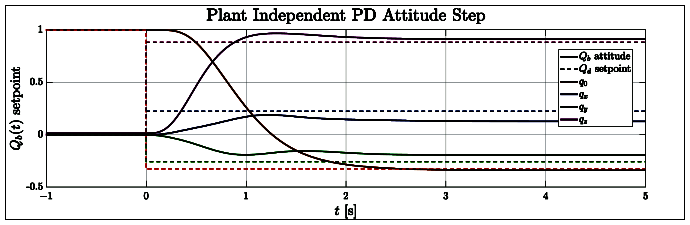
\includegraphics[width=0.8\textwidth]{graphs/PD_Diagonal_Independent_Step}
\vspace{-10pt}
\caption{Quaternion attitude step}
\label{fig:PD_Diagonal_Independent_Step}
\end{subfigure}
\begin{subfigure}{0.49\textwidth}
\centering
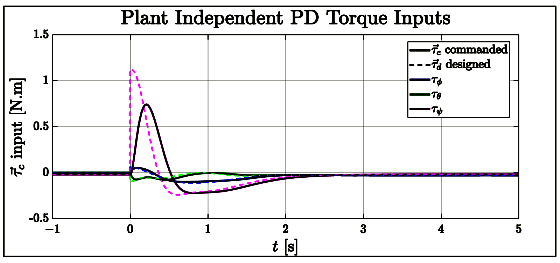
\includegraphics[width=\textwidth]{graphs/PD_Diagonal_Independent_Torque}
%\vspace{-4pt}
\caption{Plant input torques}
\label{fig:PD_Diagonal_Independent_Torque}
\end{subfigure}
\begin{subfigure}{0.49\textwidth}
\centering
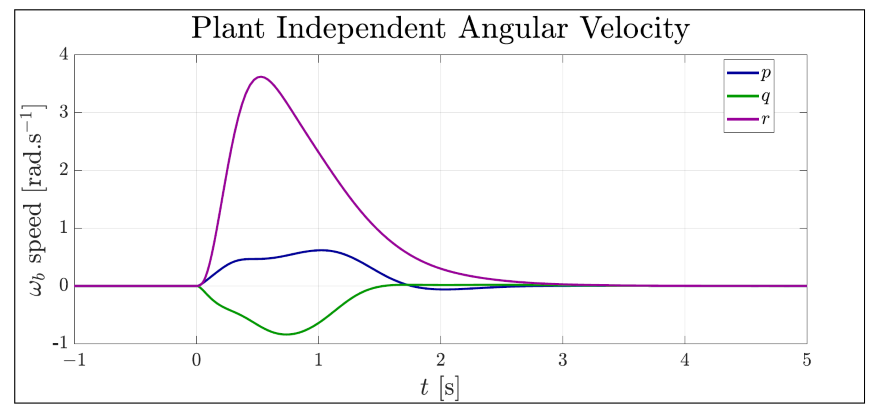
\includegraphics[width=\textwidth]{graphs/PD_Diagonal_Independent_Angular}
%\vspace{-4pt}
\caption{Angular velocity}
\label{fig:PD_Diagonal_Independent_Angular}
\end{subfigure}
\vspace{-8pt}
\caption{Independent diagonal PD}
\vspace{-20pt}
\end{figure}
%====================================================
\subsubsection{Dependent Performance}
\label{subsubsec:simulation.atttiude.pd.dependent}
%====================================================
The inclusion of a plant independent PD controller is purely for the sake of contrition; showing that plant dependency is needed to account for steady state trajectory errors (Fig:\ref{fig:independent_diagonal_trjaectory}). Those same controller coefficients from Eq:\ref{eq:optimized-pd-independent} are now used to test the controller dependent case; wherein the controller compensates for plant dynamics in Eq:\ref{eq:simulation-attitde-pd} with a feedback terms. The standard quaternion attitude step is shown in Fig:\ref{fig:PD_Diagonal_Dependent_Step} for the plant dependent case. The attitude settles in $t_{95}=3.0764~[\text{s}]$ with a dynamic response much the same as that of the independent case, Fig:\ref{fig:PD_Diagonal_Independent_Step}. However the dependent controller removes steady state tracking errors. The torque input is well still within the feasible range; not saturating any actuators. The difference is that at steady state the plant's torque input is marginally offset from zero, compensating for the previous steady state error.
\par
\begin{figure}[htbp]
\vspace{-10pt}
\centering
\begin{subfigure}{\textwidth}
\centering
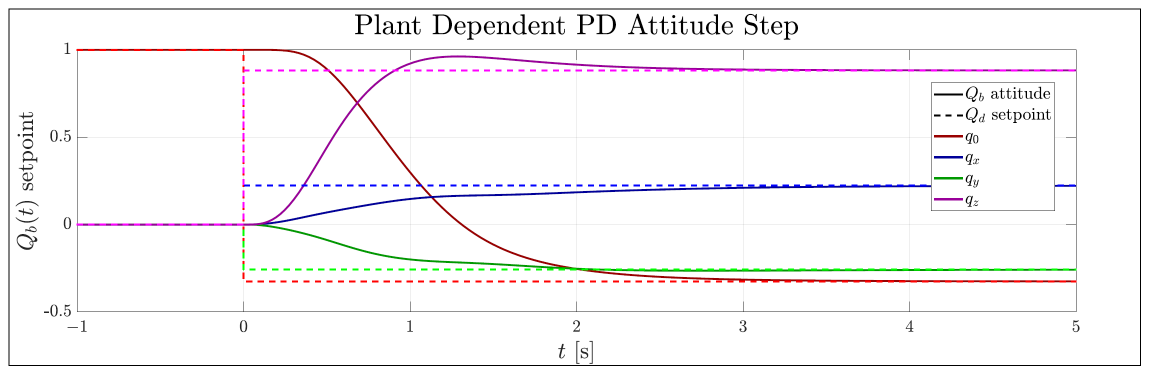
\includegraphics[width=0.8\textwidth]{graphs/PD_Diagonal_Dependent_Step}
\vspace{-6pt}
\caption{Quaternion attitude step}
\label{fig:PD_Diagonal_Dependent_Step}
\end{subfigure}
\begin{subfigure}{0.49\textwidth}
\centering
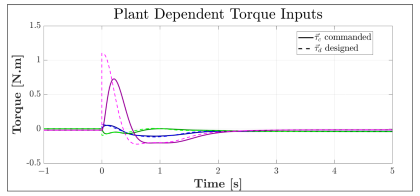
\includegraphics[width=\textwidth]{graphs/PD_Diagonal_Dependent_Torque}
\caption{Plant input torques}
\label{fig:PD_Diagonal_Dependent_Torque}
\end{subfigure}
\begin{subfigure}{0.49\textwidth}
\centering
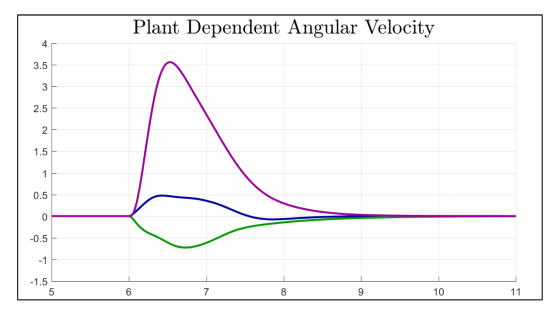
\includegraphics[width=\textwidth]{graphs/PD_Diagonal_Dependent_Angular}
\caption{Angular velocity}
\label{fig:PD_Diagonal_Dependent_Angular}
\end{subfigure}
\vspace{-8pt}
\caption{Dependent diagonal PD}
\vspace{-18pt}
\end{figure}
%====================================================
\subsubsection{Symmetric Controller Performance}
\label{subsubsec:simulation.atttiude.pd.3x3}
%====================================================
The last PD structured attitude controller considers both coefficient matrices with non-zero off-diagonal skew elements. Eq:\ref{eq:simulation-attitde-pd-symmetric-coefficients} shows the structure of both symmetric matrices and how their optimization positions are chosen. The optimized coefficients are then found to be:
\begin{equation}\label{eq:optimized-pd-symmetric}
K_p = \begin{bmatrix*}[l]
5.9157 & 0.4165 & 0.4714\\
0.4165 & 7.3141 & 0.4945\\
0.4714 & 0.4945 & 7.3135
\end{bmatrix*}
~~\text{and}~~K_d = \begin{bmatrix*}[l]
17.4318 & 0.45311 & 0.15258\\
0.45311 & 15.3569 & 0.57719\\
0.15258 & 0.57719 & 26.3436
\end{bmatrix*}
\end{equation}
The first notable difference of the symmetric controller is it's effective gain, applied by Eq:\ref{eq:optimized-pd-symmetric} to the error in Eq:\ref{eq:simulation-attitde-pd}, is significantly larger than the gain in Eq:\ref{eq:optimized-pd-independent}. The off-diagonal elements are tending towards linearizing the induced gyroscopic cross-coupled torque terms in feedback, Eq:\ref{eq:quaternion-states-angular}. The step response of the optimized symmetric PD controller is shown in Fig:\ref{fig:PD_3x3_Dependent_Step}. The increased effective gain in Eq:\ref{eq:optimized-pd-symmetric} results in larger overshoot and a slower settling time, $t_{95}=3.2993~[\text{s}]$. Neither greater commanded torque, Fig:\ref{fig:PD_3x3_Dependent_Torque}, nor an increased angular velocity spike, Fig:\ref{fig:PD_3x3_Dependent_Angular} are altogether unexpected consequences of a more aggressive control law. The increased number of coefficients to be tuned simply mean that optimization to produce Eq:\ref{eq:optimized-pd-symmetric} was perhaps not as effective at interval reduction of step errors than the diagonal Eq:\ref{eq:optimized-pd-independent}.
\newpage
\begin{figure}[htbp]
\centering
\begin{subfigure}{\textwidth}
\centering
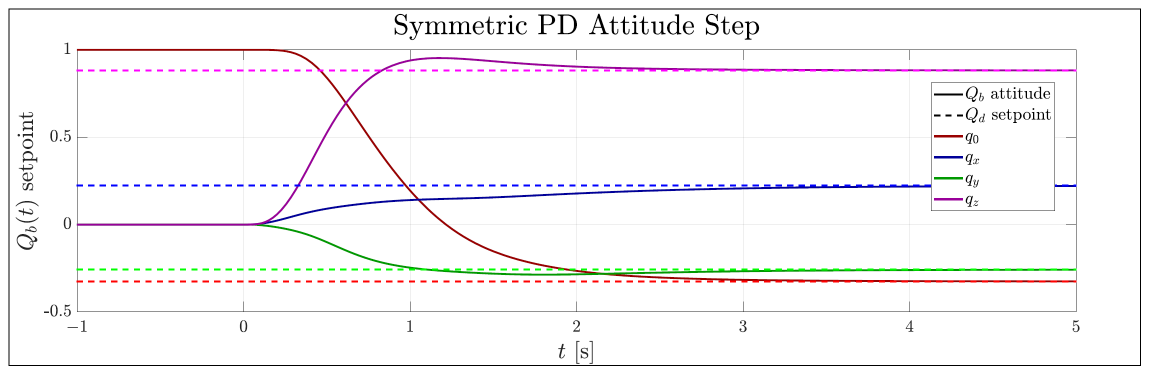
\includegraphics[width=0.8\textwidth]{graphs/PD_3x3_Dependent_Step}
\vspace{-8pt}
\caption{Quaternion attitude step}
\label{fig:PD_3x3_Dependent_Step}
\end{subfigure}
\begin{subfigure}{0.49\textwidth}
\vspace{4pt}
\centering
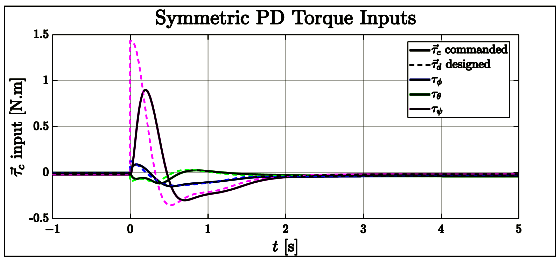
\includegraphics[width=\textwidth]{graphs/PD_3x3_Dependent_Torque}
\caption{Plant input torques}
\label{fig:PD_3x3_Dependent_Torque}
\end{subfigure}
\begin{subfigure}{0.49\textwidth}
\centering
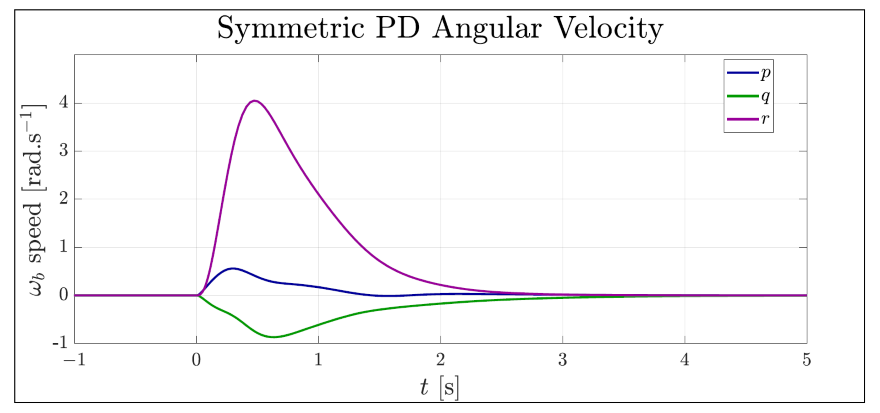
\includegraphics[width=\textwidth]{graphs/PD_3x3_Dependent_Angular}
\caption{Angular velocity}
\label{fig:PD_3x3_Dependent_Angular}
\end{subfigure}
\caption{Dependent symmetric PD}
\end{figure}
%====================================================
\subsection{Auxilliary Plant Controller}
\label{subsec:simulation.attitude.xpd}
%====================================================
The first of two the exponentially stabilizing controllers is the Auxiliary Plant controller from Sec:\ref{subsubsec:control.attitude.controllers.auxpd}. Recalling that controller structure from Eq:\ref{eq:control-aux-pd}, with Auxiliary plants defined in Eq:\ref{eq:aux-pd-1} and Eq:\ref{eq:aux-pd-2}:
\begin{equation}\label{eq:simulation-attitude-auxpd}
\vec{\tau}_{_{XPD}}=\underbrace{\Gamma_2{\widetilde{\Omega}}+\Gamma_3\vec{q}_e-J_b(u)\dot{\bar{\Omega}}}_{Independent}+\underbrace{\vec{\omega}_b\times J_b(u)\vec{\omega}_b+\hat{\tau}_b(u)-\vec{\tau}_g-\vec{\tau}_Q}_{Compensation}~~~~\in\mathcal{F}^{b}
\end{equation}
In Eq:\ref{eq:simulation-attitude-auxpd} both coefficients $\Gamma_2$ and $\Gamma_3$ are $3\times 3$ diagonal matrices; whereas $\Gamma_1$ is a symmetrical $3\times 3$ gain matrix. Those coefficients are then structured as follows:
\begin{multline}\label{eq:simulation-attitde-auxpd-coefficients}
\Gamma_1\triangleq \begin{bmatrix}
\Gamma_1(1) & \Gamma_1(4) & \Gamma_1(5)\\
\Gamma_1(4) & \Gamma_1(2) & \Gamma_1(6)\\
\Gamma_1(5) & \Gamma_1(6) & \Gamma_1(3)
\end{bmatrix}~,~~
\Gamma_2\triangleq \begin{bmatrix}
\Gamma_2(1) & 0 & 0\\
0 &\Gamma_2(2) & 0\\
0 & 0 & \Gamma_2(3)
\end{bmatrix}
\\
~~\text{and}~~\Gamma_3\triangleq \begin{bmatrix}
\Gamma_3(1) & 0 & 0\\
0 & \Gamma_3(2) & 0\\
0 & 0 & \Gamma_3(3)
\end{bmatrix}
\end{multline}
Global and local optimum coefficient swarm positions are found from the error state components on which the particular coefficients act. The first gain matrix $\Gamma_1$ acts on both $\vec{q}_e$ and $\vec{\omega}_e$ so it's local errors are best performance positions for the global error. The remaining two gain matrices $\Gamma_2$ and $\Gamma_3$ act on $\vec{q}_e$ and $\vec{\omega}_e$ respectively. The local best swarm positions are then found:
\begin{subequations}
\begin{equation}
\vec{P}_{Best}\equiv
\begin{bmatrix}
\Gamma_1(1)\Rightarrow \min \vec{\zeta}_{_{XPD}}(1) & \Gamma_1(4)\Rightarrow\min\vec{\zeta}_{_{XPD}}(1)\&\& \vec{\zeta}_{_{XPD}}(2)\\
\Gamma_1(2)\Rightarrow \min \vec{\zeta}_{_{PXD}}(2) & \Gamma_1(5)\Rightarrow\min\vec{\zeta}_{_{XPD}}(1)\&\& \vec{\zeta}_{_{XPD}}(3)\\
\Gamma_1(3)\Rightarrow \min \vec{\zeta}_{_{XPD}}(3) & \Gamma_1(6)\Rightarrow\min\vec{\zeta}_{_{XPD}}(2)\&\& \vec{\zeta}_{_{XPD}}(3)\\
\Gamma_2(1)\Rightarrow \min \vec{q}_e(1) & \Gamma_3(1)\Rightarrow\min\vec{\omega}_e(1)\\
\Gamma_2(2)\Rightarrow \min \vec{q}_e(2) & \Gamma_3(2)\Rightarrow\min\vec{\omega}_e(2)\\
\Gamma_2(3)\Rightarrow \min \vec{q}_e(3) & \Gamma_3(3)\Rightarrow\min\vec{\omega}_e(3)\\
\end{bmatrix}
\end{equation}
The position of the globally best performing swarm is found similarly:
\begin{equation}
\vec{G}_{Best}\equiv
\begin{bmatrix}
\Gamma_1(1)\Rightarrow \min \vec{\zeta}_{_{XPD}}(1) & \Gamma_1(4)\Rightarrow\min\vec{\zeta}_{_{XPD}}(1)\&\& \vec{\zeta}_{_{XPD}}(2)\\
\Gamma_1(2)\Rightarrow \min \vec{\zeta}_{_{PXD}}(2) & \Gamma_1(5)\Rightarrow\min\vec{\zeta}_{_{XPD}}(1)\&\& \vec{\zeta}_{_{XPD}}(3)\\
\Gamma_1(3)\Rightarrow \min \vec{\zeta}_{_{XPD}}(3) & \Gamma_1(6)\Rightarrow\min\vec{\zeta}_{_{XPD}}(2)\&\& \vec{\zeta}_{_{XPD}}(3)\\
\Gamma_2(1)\Rightarrow \min \vec{\zeta}_{_{XPD}}(1) & \Gamma_3(1)\Rightarrow\min\vec{\zeta}_{_{XPD}}(1)\\
\Gamma_2(2)\Rightarrow \min \vec{\zeta}_{_{XPD}}(2) & \Gamma_3(2)\Rightarrow\min\vec{\zeta}_{_{XPD}}(2)\\
\Gamma_2(3)\Rightarrow \min \vec{\zeta}_{_{XPD}}(3) & \Gamma_3(3)\Rightarrow\min\vec{\zeta}_{_{XPD}}(3)\\
\end{bmatrix}
\end{equation}
\end{subequations} 
The optimized control coefficients, after $tx=1000$ iterations, are as follows:
\begin{multline}\label{eq:optimized-auxpd}
\Gamma_1=\begin{bmatrix*}[r]
3.5924 & -0.2457 & -0.02770\\
-0.2457 & 3.0666 & -0.06023\\
-0.02770 & -0.0602 & 3.3809
\end{bmatrix*}~,~~\Gamma_2=\begin{bmatrix*}[r]
4.6943 & 0 & 0\\
0 & 4.1642 & 0\\
0 & 0 & 6.4109
\end{bmatrix*}\\
~~\text{and}~~\Gamma_3=\begin{bmatrix*}[r]
1.1007 & 0 & 0\\
0 & 1.3369 & 0 \\
0 & 0 & 1.1331
\end{bmatrix*}
\end{multline}
Besides from the stronger exponential stability, another distinctive feature of Auxilliary Controller (Eq:\ref{eq:simulation-attitde-auxpd-coefficients}) is the significant added complexity or stiffness in the control structure. Every simulation iteration in the optimizer took notably longer to complete than the simpler PD controller; typically in the order of 70-80\% longer simulation times per step test. The quaternion attitude step response is shown in Fig:\ref{fig:XPD_Step}, settling in $t_{95}=2.3688~[\text{s}]$ which is significantly faster than previous tested controllers. That improved response time does, however, come at the cost of larger input torques, shown in Fig:\ref{fig:XPD_Torque}. Moreover the angular velocity step $\vec{\omega}_b$ in Fig:\ref{fig:XPD_Angular} is significantly larger than that of previous controllers, but with a smoother derivative applied to it\ldots
\par
\begin{figure}[hbtp]
\vspace{-8pt}
\centering
\begin{subfigure}{\textwidth}
\centering
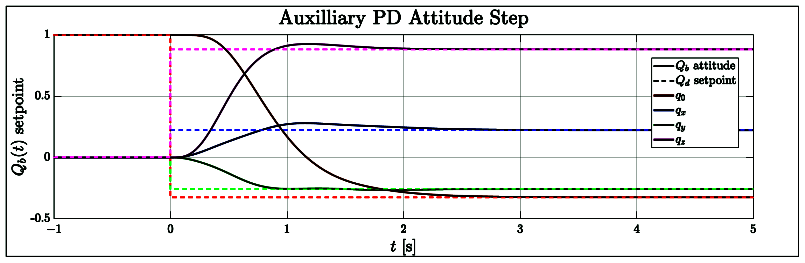
\includegraphics[width=0.8\textwidth]{graphs/XPD_Step}
\vspace{-8pt}
\caption{Quaternion attitude step}
\label{fig:XPD_Step}
\end{subfigure}
\begin{subfigure}{0.49\textwidth}
\centering
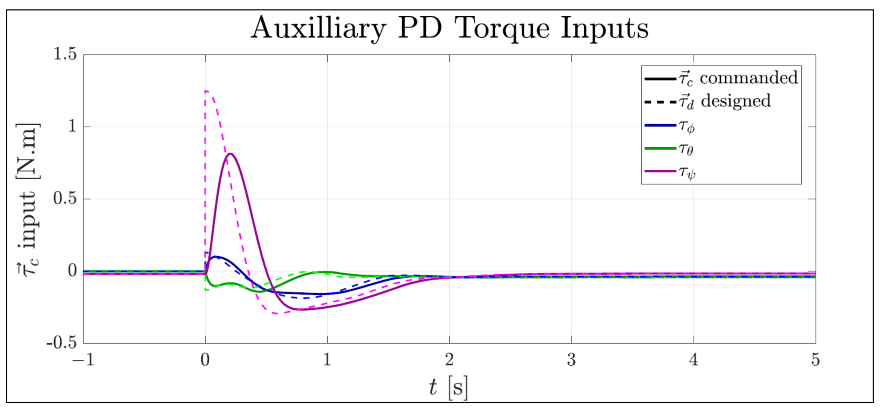
\includegraphics[width=\textwidth]{graphs/XPD_Torque}
\vspace{-12pt}
\caption{Plant input torques}
\label{fig:XPD_Torque}
\end{subfigure}
\begin{subfigure}{0.49\textwidth}
\centering
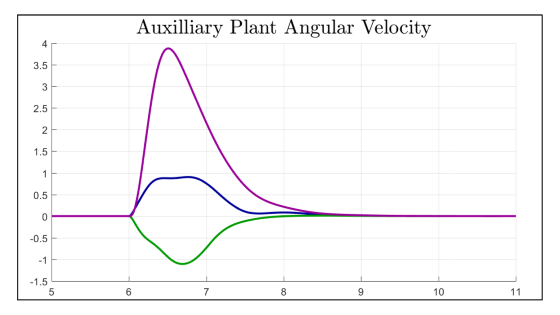
\includegraphics[width=\textwidth]{graphs/XPD_Angular}
\vspace{-12pt}
\caption{Angular velocity}
\label{fig:XPD_Angular}
\end{subfigure}
\vspace{-6pt}
\caption{Auxilliary plant controller}
\vspace{-4pt}
\end{figure}
In spite of the significantly improved settling time the Auxilliary plant controller achieves (23\% faster), the commanded and applied input torques are not as aggressive as those applied by the higher gain symmetrical PD controller (Fig:\ref{fig:PD_3x3_Dependent_Torque}). This concisely demonstrates the superiority of an exponentially stabilizing control law over a typical asymptotically stable alternative\ldots
%====================================================
\subsection{Ideal and Adaptive Backstepping Controllers}
%====================================================
The second exponentially stabilizing controller and final attitude controller to be tested is the Ideal Backstepping Controller. Both Ideal and Adaptive backstepping controllers use the same error coefficients; the difference in structure between the two is an adaptive disturbance observer. That observer estimates compensation terms introduced into the Adaptive Backstepping controller to improve robust stability. Reiterating the IBC structure from Eq:\ref{eq:control-ibc}:
\begin{equation}\label{eq:simulation-attitude-ibc}
=\underbrace{J_b(u)\Big((\Gamma_1\Gamma_2+1)\vec{q}_e-\Gamma_2\vec{\omega}_b+\Gamma_1\dot{\vec{q}}_e \Big)}_{\text{Ideal backstepping}}
+\underbrace{\vec{\omega}_b\times J_b(u)\vec{\omega}_b+\hat{\tau}_b(u)-\vec{\tau}_g-\vec{\tau}_Q}_{\text{Compenstation}}~~~~\in\mathcal{F}^{b}
\end{equation}
Wherein the gain matrices $\Gamma_1$ and $\Gamma_2$ are both positive symmetrical $3\times 3$ coefficient matrices:
\begin{equation}\label{eq:simulation-attitde-ibc-coefficients}
\Gamma_1\triangleq \begin{bmatrix}
\Gamma_1(1) & \Gamma_1(4) & \Gamma_1(5)\\
\Gamma_1(4) & \Gamma_1(2) & \Gamma_1(6)\\
\Gamma_1(5) & \Gamma_1(6) & \Gamma_1(3)
\end{bmatrix}
~~\text{and}~~
\Gamma_2\triangleq \begin{bmatrix}
\Gamma_2(1) & \Gamma_2(4) & \Gamma_2(5)\\
\Gamma_2(4) & \Gamma_2(2) & \Gamma_2(6)\\
\Gamma_2(5) & \Gamma_2(6) & \Gamma_2(3)
\end{bmatrix}
\end{equation}
However, both coefficient matrices act on the two error vectors $\vec{q}_e$ and $\vec{\omega}_e$. Trying to differentiate the local and global coefficient optimum results then becomes problematic. Making both the local and global positions equivalent reduces the directed swarm search to a randomized \emph{monte carlo} trial and error method. To avoid this it was elected to prioritize $\Gamma_1$ to control the quaternion vector error $\vec{q}_e$, similarly $\Gamma_2$ was prioritized to control the angular velocity error $\vec{\omega}_e$. It then follows that global and local best positions $\vec{P}_{best}$ and $\vec{G}_{best}$ respectively are found in the way as the symmetrical PD controller, Eq:\ref{eq:simulation-attitude-pd-symmetric-best}. This means local and global positions can still be used to direct the search space:
\begin{subequations}
\begin{equation}
\vec{P}_{Best}\equiv
\begin{bmatrix}
\Gamma_1(1)\Rightarrow \min \vec{q}_e(1) & \Gamma_1(4)\Rightarrow \min \vec{q}_e(1)\&\&\vec{q}_e(2)\\
\Gamma_1(2)\Rightarrow \min \vec{q}_e(2)& \Gamma_1(5)\Rightarrow \min\vec{q}_e(1)\&\&\vec{q}_e(3) \\
\Gamma_1(3)\Rightarrow \min \vec{q}_e(3) & \Gamma_1(6)\Rightarrow \min\vec{q}_e(2)\&\&\vec{q}_e(3)\\
\Gamma_2(1)\Rightarrow \min \vec{\omega}_e(1) & \Gamma_2(4)\Rightarrow \min\vec{\omega}_e(1)\&\&\vec{\omega}_e(2)\\
\Gamma_2(2)\Rightarrow \min \vec{\omega}_e(2) & \Gamma_2(5)\Rightarrow\min\vec{\omega}_e(1)\&\&\vec{\omega}_e(3)\\
\Gamma_2(3)\Rightarrow \min \vec{\omega}_e(3)& \Gamma_2(6)\Rightarrow\min\vec{\omega}_e(2)\&\&\vec{\omega}_e(3)
\end{bmatrix}
\end{equation}
\vspace{-10pt}
\begin{equation}
\vec{G}_{Best}\equiv\begin{bmatrix}
\Gamma_1(1)\Rightarrow \min \vec{\zeta}_{_{IBC}}(1) & \Gamma_1(4)\Rightarrow\min\vec{\zeta}_{_{IBC}}(1)\&\& \vec{\zeta}_{_{IBC}}(2)\\
\Gamma_1(2)\Rightarrow \min \vec{\zeta}_{_{IBC}}(2) & \Gamma_1(5)\Rightarrow\min\vec{\zeta}_{_{IBC}}(1)\&\& \vec{\zeta}_{_{IBC}}(3)\\
\Gamma_1(3)\Rightarrow \min \vec{\zeta}_{_{IBC}}(3) & \Gamma_1(6)\Rightarrow\min\vec{\zeta}_{_{IBC}}(2)\&\& \vec{\zeta}_{_{IBC}}(3)\\
\Gamma_2(1)\Rightarrow \min \vec{\zeta}_{_{IBC}}(1) & \Gamma_2(4)\Rightarrow\min\vec{\zeta}_{_{IBC}}(1)\&\& \vec{\zeta}_{_{IBC}}(2)\\
\Gamma_2(2)\Rightarrow \min \vec{\zeta}_{_{IBC}}(2) & \Gamma_2(5)\Rightarrow\min\vec{\zeta}_{_{IBC}}(1)\&\& \vec{\zeta}_{_{IBC}}(3)\\
\Gamma_2(3)\Rightarrow \min \vec{\zeta}_{_{IBC}}(3) & \Gamma_2(6)\Rightarrow\min\vec{\zeta}_{_{IBC}}(2)\&\& \vec{\zeta}_{_{IBC}}(3)\\
\end{bmatrix}
\end{equation}
\end{subequations}
The optimized then yielded the following two sets of gain coefficient matrices:
\begin{equation}\label{eq:optimized-IBC}
\Gamma_1 = \begin{bmatrix*}[r]
5.86306 & 0.0515342 & 1.02209\\
0.0515342 & 13.8375 & 0.853279\\
1.02209 & 0.853279 & 11.9644
\end{bmatrix*}
~~\text{and}~~
\Gamma_2 = \begin{bmatrix*}[r]
9.1127 & 0.28871 & 0.13528\\
0.28871 & 6.8389 & 0.19714\\
0.13528 & 0.18714 & 2.5294
\end{bmatrix*}
\end{equation}
\begin{figure}[hbtp]
\vspace{-20pt}
\centering
\begin{subfigure}{\textwidth}
\centering
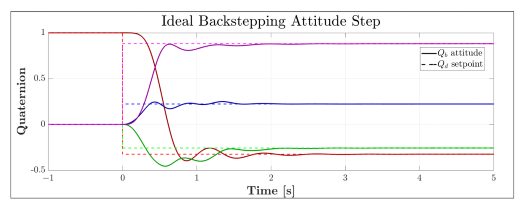
\includegraphics[width=0.8\textwidth]{graphs/IBC_Step}
\vspace{-10pt}
\caption{Quaternion attitude step}
\label{fig:IBC_Step}
\end{subfigure}
\vspace{-20pt}
\end{figure}
\newpage
\begin{figure}[htbp]\ContinuedFloat
\begin{subfigure}{0.49\textwidth}
\centering
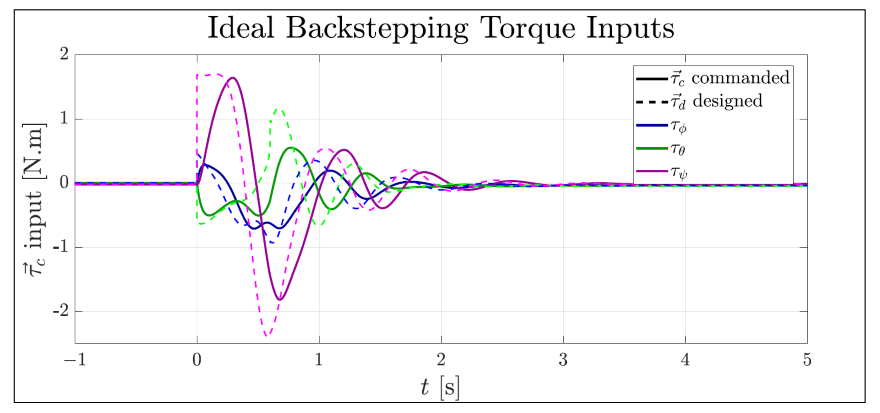
\includegraphics[width=\textwidth]{graphs/IBC_Torque}
\caption{Plant input torques}
\label{fig:IBC_Torque}
\end{subfigure}
\begin{subfigure}{0.49\textwidth}
\centering
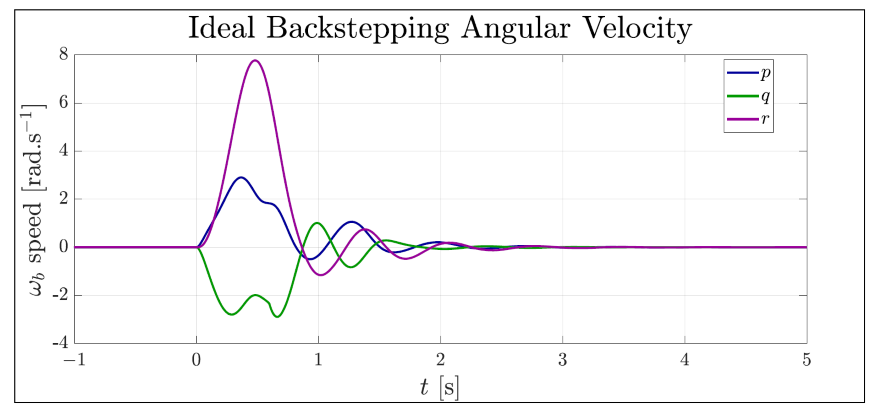
\includegraphics[width=\textwidth]{graphs/IBC_Angular}
\caption{Angular velocity}
\label{fig:IBC_Angular}
\end{subfigure}
\vspace{-6pt}
\caption{Independent diagonal PD}
\vspace{-12pt}
\end{figure}
\par
The regular attitude step's response in Fig:\ref{fig:IBC_Step} shows a dramatically faster response, with notable oscillations at the settling point. The step settles in $t_{95}=1.6403~[\text{s}]$; almost twice as fast as a basic PD controller but the commanded control inputs in Fig:\ref{fig:IBC_Torque} are the largest of all the controllers. Out of each control law suggested the IBC is by far the most aggressive which results sizeable and perhaps unsatisfactory overshoot. Furthermore the commanded angular velocity changes for the IBC controller are, on average, twice the size of the previous control laws. The Adaptive backstepping controller is tested and discussed later in Sec:\ref{subsec:simulation.disturbance.torque} in the context of robust trajectory stability; rather than controller stepped performances here\ldots 
%====================================================
\section{Position Controllers}
\label{sec:simulation.position}
%====================================================
Following the attitude controller optimization, a similar approach was applied to the two proposed position control laws (in Sec:\ref{sec:control.position}). It is important to specify that, for position controller optimization, a plant dependent diagonal PD attitude controller (Sec:\ref{subsubsec:simulation.atttiude.pd.dependent}) was used to stabilize the coupled attitude dynamics. To test each position controller coefficient swarm's performance the attitude setpoint was kept at a constant $Q_d=[1~\vec{0}\hspace{2pt}]^T$, while various position setpoints were applied. Moreover the same basic pseudo inversion allocator (Sec:\ref{subsec:allocation.allocators.inverse}) was used for position control to allocate out the virtual control input $\vec{\nu}_d$/ Each position setpoint is defined in the inertial frame:
\begin{equation}
\vec{\mathcal{E}}_d(t)\triangleq\begin{bmatrix}
X_d(t)&
Y_d(t)&
Z_d(t)
\end{bmatrix}^T
~~~~\in\mathcal{F}^{I}
\end{equation}
A collection of position setpoints were tested where each setpoint was positioned on the surface of a sphere at a radius of $C=5~[\text{m}]$ away from a central starting point. That starting position was consistently tested at $\vec{\mathcal{E}}_0=[5~5~5]^{T}~[\text{m}]$, relative to the inertial frame's origin. Each setpoint was then distanced away from $\vec{\mathcal{E}}_0$ as per a rotated radial arm:
\begin{equation}
\vec{\mathcal{E}}_d(t)=\vec{\mathcal{E}}_0+R_y(\theta_{y})R_x(\phi_{x})\begin{bmatrix}
0 & 0 & 5
\end{bmatrix}^T
\end{equation}
Both test angles $\phi_x$ and $\theta_y$ rotate the radial arm  $C$ for a range $\phi_x\in[-180\text{\textdegree}:180\text{\textdegree}]$ and $\theta_y\in[-90\text{\textdegree}:90\text{\textdegree}]$; both at $30~\text{\textdegree}$ increments. That results in test space position surface illustrated in Fig:\ref{fig:position-setpoint}, with a total of 91 position setpoints to test. Performance of each position step was evaluated with another ITAE integral for the position and translational velocity errors, both transformed into the \emph{body frame}, $\mathcal{F}^{b}$. Again the simulation was given $t=15~[\text{s}]$ to reach it's settling point when stepped from the starting point.
\begin{equation}\label{eq:position-performance}
\vec{\zeta}_{\mathcal{E}}=C_{X}\int_{t=0}^{15}t|\vec{X}_e(t)|.dt+C_{v}\int_{t=0}^{15}t|\vec{v}_e(t)|.dt
\end{equation}
Weighting coefficients $C_X$ and $C_v$ prioritize position and velocity errors respectively, both were weighted equally such that $C_X=C_v=1$. Each swarm was then tested 91 times and the resultant cost of Eq:\ref{eq:position-performance} was averaged for an overall performance metric. Only plant dependent compensating position controllers were considered and optimized for the position control loop. Not compensating for the graviational force acceleration applied to the vehicle in it's differential equation of motion, Eq:\ref{eq:quaternion-states-acceleration}, \emph{would} result in instability. To compare the relative performance of position controllers a constant step test was applied in both cases:
\begin{equation}\label{eq:position-step}
\vec{\mathcal{E}}_d=\begin{bmatrix}
X_d&
Y_d&
Z_d
\end{bmatrix}^T=\begin{bmatrix}
7.5&
4&
3
\end{bmatrix}^T~~[\text{m}],~\in\mathcal{F}^{I}
\end{equation}
\par
\begin{figure}[htbp]
\centering
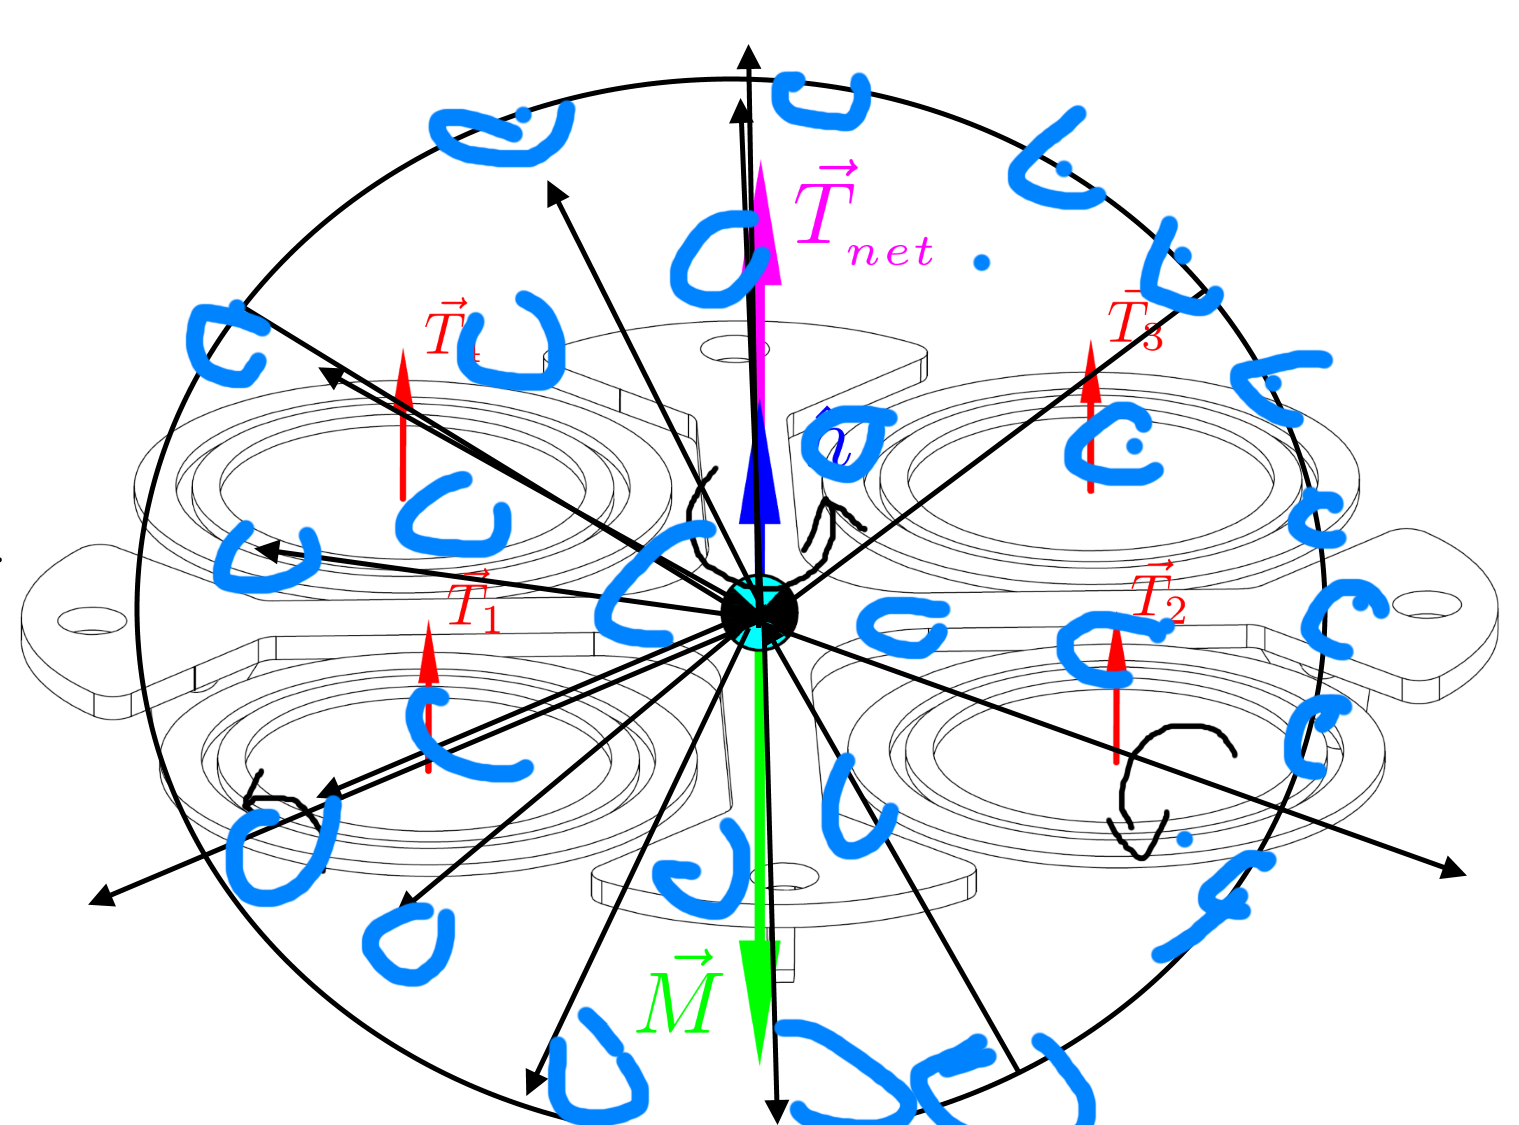
\includegraphics[width=0.7\textwidth]{figs/position-setpoint}
\caption{Position setpoint workspace}
\label{fig:position-setpoint}
\end{figure}
\par
%====================================================
\subsection{PD}
\label{subsec:simulation.position.pd}
%====================================================
The reference case for position control is the Proportional-Derivative controller, presented in Sec:\ref{subsec:control.position.pd}. The PD position controller designs a control force input, from Eq:\ref{eq:position-pd}:
\begin{equation}
\vec{F}_{_{PD}}=K_p\vec{X}_e + K_d\dot{\vec{X}}_e + \vec{\omega}_b\times m_b\vec{v}_b-m_b\vec{G}_b~~~~\in\mathcal{F}^{b}
\end{equation}
Where both $K_p$ and $K_d$ are diagonal gain coefficient matrices. The introduction of symmetric coefficients did not yield in improvements for the attitude plant in Sec:\ref{subsubsec:simulation.atttiude.pd.3x3} so it was not investigated here in the context of position control. The two gain coefficients for the PD controller are structured as follows:
\begin{equation}\label{eq:simulation-attitde-pd-diagonal-coefficients}
K_p\triangleq \begin{bmatrix}
K_p(1) & 0 & 0\\
0 & K_p(2) & 0\\
0 & 0 & K_p(3)
\end{bmatrix}
~~\text{and}~~K_d\triangleq \begin{bmatrix}
K_d(1) & 0 & 0\\
0 & K_d(2) & 0\\
0 & 0 & K_d(3)
\end{bmatrix}
\end{equation}
Each coefficient matrix acts on the position error vector, $\vec{X}_e$, and the velocity error vector, $\vec{v}_e$, independently. As a result the local and global coefficient optimum positions are selected simply as:
\begin{equation}
\vec{P}_{Best}\equiv
\begin{bmatrix}
K_p(1)\Rightarrow \min \vec{X}_e(1)\\
K_p(2)\Rightarrow \min \vec{X}_e(2)\\
K_p(3)\Rightarrow \min \vec{X}_e(3)\\
K_d(1)\Rightarrow \min \vec{v}_e(1)\\
K_d(2)\Rightarrow \min \vec{v}_e(2)\\
K_d(3)\Rightarrow \min \vec{v}_e(3)
\end{bmatrix}~~\text{and}~~\vec{G}_{Best}\equiv\begin{bmatrix}
K_p(1)\Rightarrow \min \vec{\zeta}_{_{PD}}(1)\\
K_p(2)\Rightarrow \min \vec{\zeta}_{_{PD}}(2)\\
K_p(3)\Rightarrow \min \vec{\zeta}_{_{PD}}(3)\\
K_d(1)\Rightarrow \min \vec{\zeta}_{_{PD}}(1)\\
K_d(2)\Rightarrow \min \vec{\zeta}_{_{PD}}(2)\\
K_d(3)\Rightarrow \min \vec{\zeta}_{_{PD}}(3)
\end{bmatrix}
\end{equation}
The following optimized coefficients were then produced:
\begin{equation}\label{eq:optimized-position-pd}
K_p = \begin{bmatrix}
2.4167 & 0 & 0\\
0 & 2.1557 & 0\\
0 & 0 & 2.5904
\end{bmatrix}
~~\text{and}~~K_d = \begin{bmatrix}
3.4794 & 0 & 0\\
0 & 3.3846 & 0\\
0 & 0 & 3.8698
\end{bmatrix}
\end{equation}
The inertial position step had a response shown in Fig:\ref{fig:PD_Position_Step}; stepping from the initial position to the setpoint(s) described in Eq:\ref{eq:attitude-step-position}. The position step settled in $t_{95}=4.007~[\text{s}]$ without any overshoot. Not shown but still considered is the effect a position step has on the attitude plant's stability, which still remained stable at the origin with no deviations. Because the attitude setpoint is $Q_d=[1~\vec{0}]^T$; almost all the force requirement in steady state is to oppose the gravitational downward force acting on the body, Fig:\ref{fig:PD_Position_Force}.
\begin{figure}[htbp]
\vspace{-12pt}
\centering
\begin{subfigure}{\textwidth}
\centering
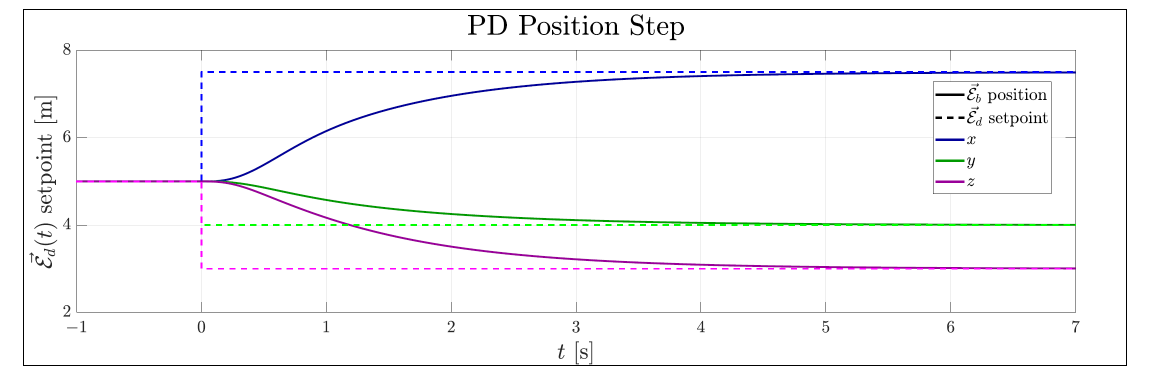
\includegraphics[width=0.8\textwidth]{graphs/PD_Position_Step}
\vspace{-6pt}
\caption{Position step}
\label{fig:PD_Position_Step}
\end{subfigure}
\begin{subfigure}{0.49\textwidth}
\centering
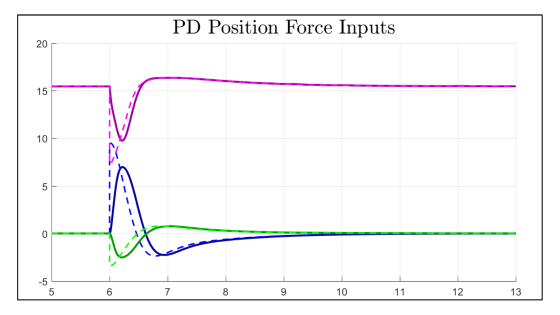
\includegraphics[width=\textwidth]{graphs/PD_Position_Force}
\caption{Plant input forces}
\label{fig:PD_Position_Force}
\end{subfigure}
\begin{subfigure}{0.49\textwidth}
\centering
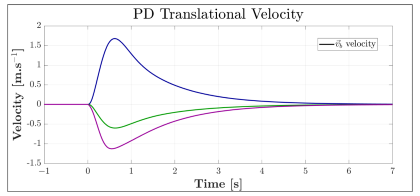
\includegraphics[width=\textwidth]{graphs/PD_Position_Velocity}
\caption{Position translational velocity}
\label{fig:PD_Position_Velocity}
\end{subfigure}
\caption{Position PD}
\vspace{-24pt}
\end{figure}
%====================================================
\subsection{Ideal and Adaptive Position Backstepping}
\label{subsec:simulation.position.pd}
%====================================================
The second and final position controller to be tested is the Ideal Backstabbing controller, the only exponentially stable position control law proposed. As is the case with attitude IBC controller, the coefficients selected for the Ideal Backstepping case are used again for the Adaptive cases; the latter is evaluated subsequently in Sec:\ref{subsec:simulation.disturbance.force}. Recalling the position IBC structure from Sec:\ref{subsec:control.position.bacstepping}:
\begin{equation}\label{eq:simulation-position-IBC}
\vec{F}_{_{IBC}}=m_b\Big(\big(1+\Gamma_1\Gamma_2\big)\hat{z}_1-\big(\Gamma_1+\Gamma_2\big)\vec{v}_b\big)\Big)+\vec{\omega}_b\times m_b\vec{v}_b-m_b\vec{G}_b-\vec{D}_b~~~~\in\mathcal{F}^{b}
\end{equation}
The two positive symmetric coefficient gain matrices in Eq:\ref{eq:simulation-position-IBC} are structured are:
\begin{equation}\label{eq:simulation-position-diagonal-coefficients}
\Gamma_1\triangleq \begin{bmatrix}
\Gamma_1(1) & \Gamma_1(4) & \Gamma_1(5)\\
\Gamma_1(4) & \Gamma_1(2) & \Gamma_1(6)\\
\Gamma_1(5) & \Gamma_1(6) & \Gamma_1(3)
\end{bmatrix}
~~\text{and}~~\Gamma_2\triangleq \begin{bmatrix}
\Gamma_2(1) & \Gamma_2(4) & \Gamma_2(5)\\
\Gamma_2(4) & \Gamma_2(2) & \Gamma_2(6)\\
\Gamma_2(5) & \Gamma_2(6) & \Gamma_2(3)
\end{bmatrix}
\end{equation}
Both attitude and position ideal backstepping controllers have coefficients which act on both plant's error and error rates. This makes local and global coefficient position selection difficult without adversely affecting the swarm's optimization trajectory process. 
\par
Then using this first coefficient matrix $\Gamma_1$ to prioritize position tracking errors $\vec{X}_e$ and relegating $\Gamma_2$ to settle velocity errors $\vec{v}_e$; the local and global best positions are chosen as follows:
\begin{subequations}
\begin{equation}
\vec{P}_{Best}\equiv
\begin{bmatrix}
\Gamma_1(1)\Rightarrow \min \vec{\mathcal{X}}_e(1) & \Gamma_1(4)\Rightarrow \min \vec{\mathcal{X}}_e(1)\&\&\vec{\mathcal{X}}_e(2)\\
\Gamma_1(2)\Rightarrow \min \vec{\mathcal{X}}_e(2)& \Gamma_1(5)\Rightarrow \min\vec{\mathcal{X}}_e(1)\&\&\vec{\mathcal{X}}_e(3) \\
\Gamma_1(3)\Rightarrow \min \vec{\mathcal{X}}_e(3) & \Gamma_1(6)\Rightarrow \min\vec{\mathcal{X}}_e(2)\&\&\vec{\mathcal{X}}_e(3)\\
\Gamma_2(1)\Rightarrow \min \vec{v}_e(1) & \Gamma_2(4)\Rightarrow \min\vec{v}_e(1)\&\&\vec{v}_e(2)\\
\Gamma_2(2)\Rightarrow \min \vec{v}_e(2) & \Gamma_2(5)\Rightarrow\min\vec{v}_e(1)\&\&\vec{v}_e(3)\\
\Gamma_2(3)\Rightarrow \min \vec{v}_e(3)& \Gamma_2(6)\Rightarrow\min\vec{v}_e(2)\&\&\vec{v}_e(3)
\end{bmatrix}
\end{equation}
\vspace{-8pt}
\begin{equation}
\vec{G}_{Best}\equiv\begin{bmatrix}
\Gamma_1(1)\Rightarrow \min \vec{\zeta}_{_{IBC}}(1) & \Gamma_1(4)\Rightarrow\min\vec{\zeta}_{_{IBC}}(1)\&\& \vec{\zeta}_{_{IBC}}(2)\\
\Gamma_1(2)\Rightarrow \min \vec{\zeta}_{_{IBC}}(2) & \Gamma_1(5)\Rightarrow\min\vec{\zeta}_{_{IBC}}(1)\&\& \vec{\zeta}_{_{IBC}}(3)\\
\Gamma_1(3)\Rightarrow \min \vec{\zeta}_{_{IBC}}(3) & \Gamma_1(6)\Rightarrow\min\vec{\zeta}_{_{IBC}}(2)\&\& \vec{\zeta}_{_{IBC}}(3)\\
\Gamma_2(1)\Rightarrow \min \vec{\zeta}_{_{IBC}}(1) & \Gamma_2(4)\Rightarrow\min\vec{\zeta}_{_{IBC}}(1)\&\& \vec{\zeta}_{_{IBC}}(2)\\
\Gamma_2(2)\Rightarrow \min \vec{\zeta}_{_{IBC}}(2) & \Gamma_2(5)\Rightarrow\min\vec{\zeta}_{_{IBC}}(1)\&\& \vec{\zeta}_{_{IBC}}(3)\\
\Gamma_2(3)\Rightarrow \min \vec{\zeta}_{_{IBC}}(3) & \Gamma_2(6)\Rightarrow\min\vec{\zeta}_{_{IBC}}(2)\&\& \vec{\zeta}_{_{IBC}}(3)\\
\end{bmatrix}
\end{equation}
\end{subequations}
The optimized gain coefficients for $\Gamma_1$ and $\Gamma_2$ were then produced by the PSO algorithm:
\begin{equation}\label{eq:optimized-Position-IBC}
\Gamma_1 = \begin{bmatrix}
2.3409 & 0.17071 & -0.16444\\
0.17071 & 2.0493 & 0.10597\\
-0.16444 & 0.10597 & 1.7322
\end{bmatrix}
~~\text{and}~~\Gamma_2= \begin{bmatrix}
1.5287 & 0.029275 & 0.081552\\
0.029275 & 1.4214 & -0.041008\\
0.081552 & -0.041008 & 1.4753
\end{bmatrix}
\end{equation}
\par
\begin{figure}[hbtp]
\vspace{-15pt}
\centering
\begin{subfigure}{\textwidth}
\centering
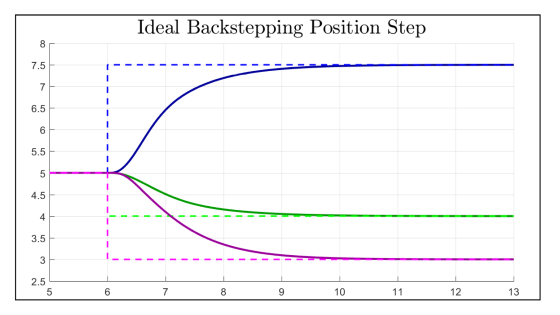
\includegraphics[width=0.8\textwidth]{graphs/IBC_Position_Step}
\caption{Position step}
\label{fig:IBC_Position_Step}
\end{subfigure}
\begin{subfigure}{0.49\textwidth}
\centering
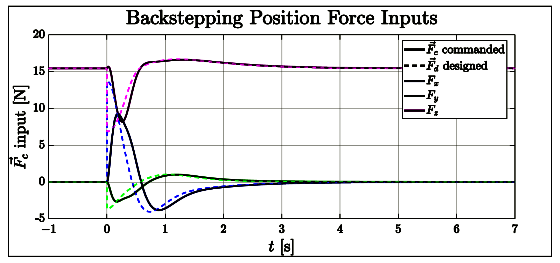
\includegraphics[width=\textwidth]{graphs/IBC_Position_Force}
\caption{Plant input forces}
\label{fig:IBC_Position_Force}
\end{subfigure}
\begin{subfigure}{0.49\textwidth}
\centering
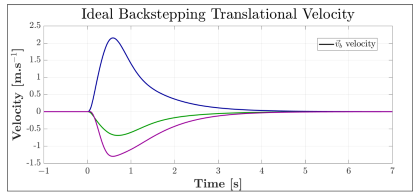
\includegraphics[width=\textwidth]{graphs/IBC_Position_Velocity}
\caption{Position translational velocity}
\label{fig:IBC_Position_Velocity}
\end{subfigure}
\vspace{-6pt}
\caption{Position Backstepping Controller}
\vspace{-8pt}
\end{figure}
\par
Fig:\ref{fig:IBC_Position_Step} shows the step response to a change in translational position setpoint. Note that the position plotted in Fig:\ref{fig:IBC_Position_Step} is the relative position in the inertial frame $\mathcal{F}^{I}$, not the backstepping input $\vec{X}_e$. The Ideal Backstepping controller settles in $t_{95}=2.987~[\text{s}]$; demonstrating the improvement exponential stability has over asymptotic stability achieved by a PD controller previously\ldots
\par
It is not unexpected that with faster settling times greater input forces are commanded, the virtual and commanded input forces in Fig:\ref{fig:IBC_Position_Force} spike to a larger degree than those previously in Fig:\ref{fig:PD_Position_Force}. The velocity step, in Fig:\ref{fig:IBC_Position_Velocity}, follows a smooth rate change.
%====================================================
\section{Set-point Control Results}
\label{sec:simulation.autopilot}
%====================================================
Each presented attitude or position controllers was respectively stable in it's own right. The trajectory used to corroborate dynamic setpoint tracking (Fig:\ref{fig:trajectory}) is not a complicated, a slow orbital velocity of $\dot{\theta}=0.5~[\text{Hz}]$ was applied such that a single orbit around $\vec{C}_0$ was completed every $120~[\text{s}]$. Two Proportional Derivative attitude controllers are tested, both with diagonal gain matrices (from Eq:\ref{eq:optimized-pd-independent}), it was shown previously that symmetric gain coefficients yield no improvements in settling times. Furthermore Sec:\ref{subsec:simulation.attitude.pd} demonstrated plant independent controllers produce steady state errors for an attitude step. The same can be said for the independent controllers trajectory tracking, shown in Fig:\ref{fig:independent_diagonal_trjaectory}. Adaptive backstepping controllers and their disturbance rejection properties are discussed next in Sec:\ref{sec:simulation.disturbnace}. 
\par
Each attitude controller was tested together with a common PD position controller, tracking the orbital XYZ position. Conversely each position controller is tested using a simple diagonal PD controller to track the attitude. The attitude controllers have an initial step to reach the orbital attitude from their starting attitude; $Q_0=[1~\vec{0}]^T$. Each control law was successful in tracking a given trajectory each with little to no error. Of coarse trajectory errors could be improved even further with higher order derivative tracking introduced into each controller ($\vec{\omega}_d\not=\vec{0}$ and $\vec{v}_d\not=\vec{0}$).
\begin{figure}[hbtp]
\vspace{-10pt}
\begin{subfigure}{\textwidth}
\centering
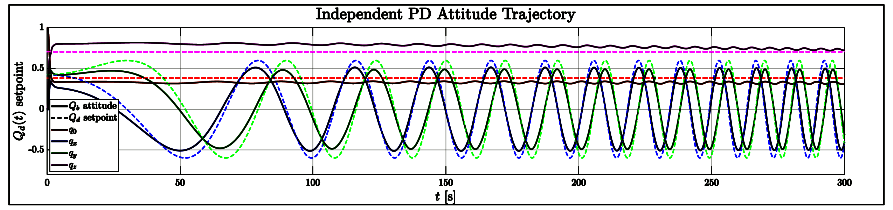
\includegraphics[width=0.8\textwidth]{graphs/PD_Diagonal_Independent_Trajectory}
\vspace{-11pt}
\caption{Independent Proportional Derivative Attitude Controller}
\label{fig:independent_diagonal_trjaectory}
\end{subfigure}
\begin{subfigure}{\textwidth}
\vspace{-3pt}
\centering
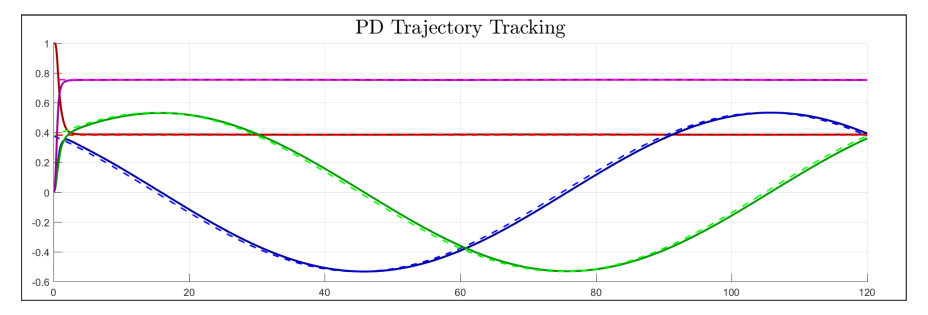
\includegraphics[width=0.8\textwidth]{graphs/PD_Diagonal_Dependent_Trajectory}
\vspace{-11pt}
\caption{Dependent Proportional Derivative Attitude Controller}
\end{subfigure}
\begin{subfigure}{\textwidth}
\vspace{-3pt}
\centering
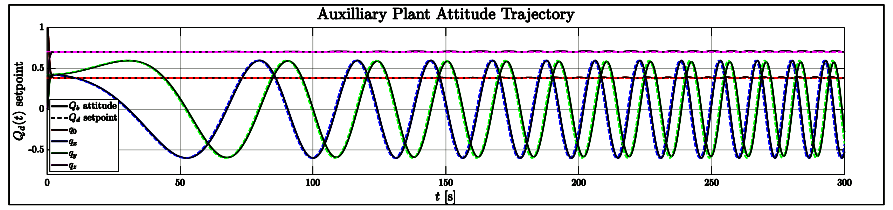
\includegraphics[width=0.8\textwidth]{graphs/XPD_Trajectory}
\vspace{-11pt}
\caption{Auxiliary Plant Attitude Controller}
\end{subfigure}
\vspace{-24pt}
\end{figure}
\par
\begin{figure}[hbtp]\ContinuedFloat
\vspace{-6pt}
\begin{subfigure}{\textwidth}
\centering
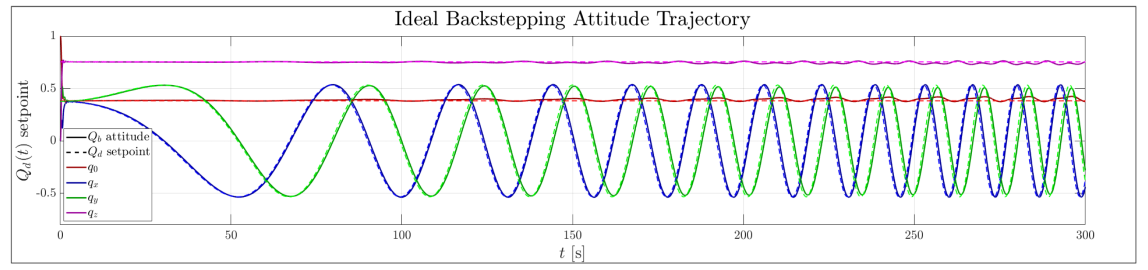
\includegraphics[width=0.8\textwidth]{graphs/IBC_Trajectory}
\vspace{-11pt}
\caption{Ideal Backstepping Controller}
\label{fig:attitude-trajectory-ibc-tracking}
\end{subfigure}
\vspace{-8pt}
\caption{Attitude Trajectory Tracking}
\label{fig:attitude-trajectory-tracking}
\vspace{-14pt}
\end{figure}
The only notable difference between theattitude controllers
plotted in Fig:\ref{fig:attitude-trajectory-tracking} is that, at the initial attitude step, the Ideal Backstepping attitude controller (Fig:\ref{fig:attitude-trajectory-ibc-tracking}) introduces some oscillations whilst settling. The independent PD controller actually tracks some trajectory, but with a steady state error.
\par
\begin{figure}[hbtp]
\vspace{-12pt}
\begin{subfigure}{\textwidth}
\centering
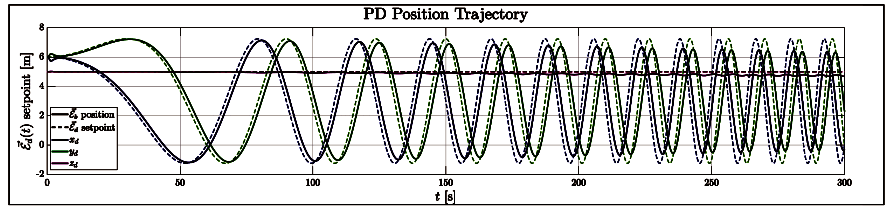
\includegraphics[width=0.8\textwidth]{graphs/PD_Position_Trajectory}
\vspace{-12pt}
\caption{Diagonal Proportional Derivative Controller}
\end{subfigure}
\begin{subfigure}{\textwidth}
\vspace{-3pt}
\centering
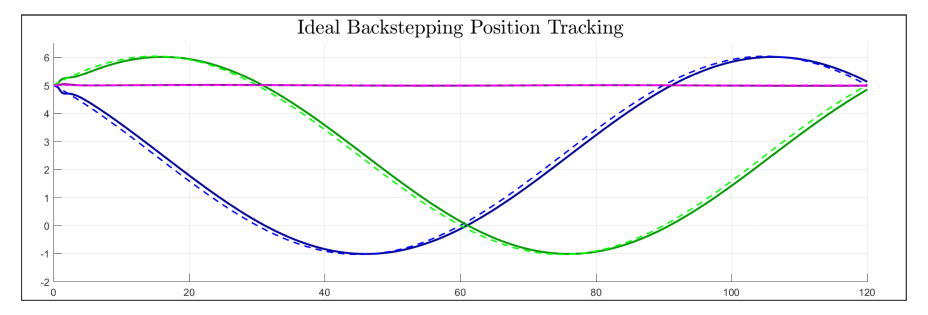
\includegraphics[width=0.85\textwidth]{graphs/IBC_Position_Trajectory}
\vspace{-12pt}
\caption{Ideal Backstepping Controller}
\end{subfigure}
\caption{Position Trajectory Tracking}
\label{fig:position-trajectory-tracking}
\vspace{-10pt}
\end{figure}
\par
There is a marginal phase lag in the position controller's trajectories, Fig:\ref{fig:position-trajectory-tracking}. Once again this is a consequence of tracking only first order setpoint; if translational velocity setpoints were applied as well that phase delay would be diminished\ldots
%====================================================
\section{Robust Stability and Disturbance Rejection}
\label{sec:simulation.disturbnace}
%====================================================
Despite deriving adaptive control laws in Sec:\ref{subsubsec:control.attitude.nonlinear.adaptivebackstep} and Sec:\ref{subsec:control.position.bacstepping} for attitude and position controllers respectively; each of the proposed controls demonstrated acceptable stability under sizeable disturbances. App:\ref{app:disturbance} shows each controller's trajectory response to uncompensated disturbances acting on the vehicle. The torque and force disturbances are described subsequently\ldots
%====================================================
\subsection{Torque Disturbance Rejection}
\label{subsec:simulation.disturbance.torque}
%====================================================
Typically  turbulence torques are difficult to define without in-depth statistical and mathematical analysis. To expedite the stability/disturbance evaluation process, torque turbulences were approximated using a Dryden Gust model,\cite{optimalgust,discretegustmodel}. Alternatively the Von Karman aerospace disturbance model(s) could be implemented but that is computationally more exhaustive.
\par
Without going into too much detail, the Dryden Wind model produces turbulence signals from white noise filtered through a specified Dryden power spectrum. That power spectrum varies as per an aircraft's orientation, altitude and translational velocity. For the aircraft and trajectory under consideration here such a disturbance model is sufficient for simulating small interference patterns. Recalling then the torque disturbance observer derived for the attitude backstepping plant, from Eq:\ref{eq:asymptotic-disturbance}:
\begin{equation}\label{eq:stability-torque-overserver}
\dot{\hat{L}}=-\Gamma_L J_b^{-1}(u)\big(\Gamma_1\vec{q}_e-\vec{\omega_b}\big)
\end{equation}
The gain adaptivity matrix $\Gamma_L$ was tuned on steady state such that the observer's error deviation from an applied torque $\vec{L}$ was minimized. That resulted in the diagonal adaptivity matrix of $\Gamma_L=diag(29.58,~28.43,~4.60)$. The approximator tracks an applied disturbance as shown in Fig:\ref{fig:torque-observer} over a disturbance range of $\pm 0.2~[\text{N.m}]$ for a short steady state test. Both pitch and roll torque approximator channels ($\phi$ and $\theta$) track the torque with a small error, the deviation from the applied torque only occurs in the $\psi$ channel about the $\hat{Z}_b$ axis\ldots
\begin{figure}[htbp]
\vspace{-12pt}
\centering
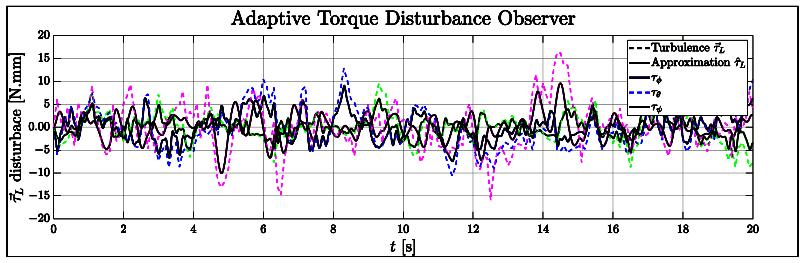
\includegraphics[width=0.8\textwidth]{graphs/torque-observer}
\vspace{-12pt}
\caption{Attitude torque disturbance observer}
\vspace{-16pt}
\label{fig:torque-observer}
\end{figure}
\par
Fig:\ref{fig:ABC_trajectory} then shows the Adaptive Backstepping controller's attitude response over the entire orbital trajectory whilst experiencing a fluctuating torque turbulence. The addition of a torque observer for compensation produces a slight improvement over an uncompensated IBC controller; shown in Fig:\ref{fig:app-attitude-ibc-dist} from App:\ref{app:disturbance}. 
\begin{figure}[hbtp]
\vspace{-6pt}
\centering
\includegraphics[width=0.8\textwidth]{graphs/ABC_trajectory}
\vspace{-12pt}
\caption{Adaptive backstepping attitude trajectory tracking}
\label{fig:ABC_trajectory}
\vspace{-16pt}
\end{figure}
\par
The cost of the disturbance approximator in the attitude plant is obviously more aggressive and greater bandwidth fluctuating input torques applied to the control plant. That could potentially reach actuator rate saturation, but for the trajectories tested here, were not saturation inducing.
%====================================================
\subsection{Disturbance Force Rejection}
\label{subsec:simulation.disturbance.force}
%====================================================
Force disturbances are similarly emulated in simulation using a Dryden Gust model for wind turbulent velocity generation. Additional a wind vector field, across the inertial frame test space, was also used to introduce a constant force offset throughout the trajectory simulation. The force disturbance observer, from Eq:\ref{eq:abc-asymptotic-position}, has an estimate update rule such that:
\begin{equation}
\dot{\hat{D}}=-m_b^{-1}\Gamma_D\Big(\Gamma_1\vec{X}_e-\vec{v}_b\Big)
\end{equation}
Where $\vec{X}_e$ is the inertial position error transformed to the body frame, $\vec{X}_e=Q_b\otimes\vec{\mathcal{E}}_e\otimes Q_b^*$. Then $\Gamma_D$ is the force disturbance observer's adaptivity gain matrix. Using the coefficients $\Gamma_D=diag(4.203,~3.840,~3.971)$ the observer tracks a force disturbance acting on the vehicle over a range of $-4\rightarrow 8~[N]$. Fig:\ref{fig:force-observer} shows how the force observer adapts to the variable force turbulence applied, the plot is taken over an entire simulation (until $t=120~[\text{s}]$) to illustrate the vector field effects.
\begin{figure}[hbtp]
\vspace{-6pt}
\centering
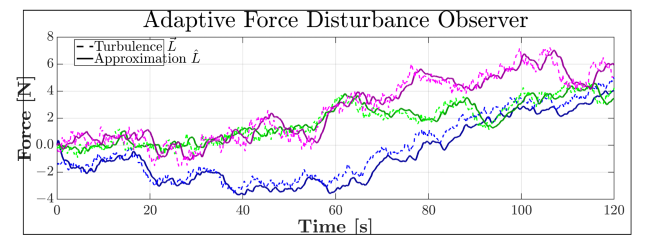
\includegraphics[width=0.8\textwidth]{graphs/force-observer}
\vspace{-12pt}
\caption{Position force disturbance observer}
\label{fig:force-observer}
\vspace{-16pt}
\end{figure}
\par
The position adaptive backstepping controller then tracks the inertial frame trajectory as shown in Fig:\ref{fig:ABC_Position_Trajectory}. Again improving the trajectory tracking performance slightly when compared to the Ideal backstepping case from Fig:\ref{fig:app-position-ibc-dist}; but even without adaptive disturbance compensation, the plant is stable throughout the trajectory albeit somewhat noisy. The addition of a vector force field results in a fluctuating offset error from the trajectory, despite the adaptive compensation applied to the control loop.
\begin{figure}[hbtp]
\vspace{-6pt}
\centering
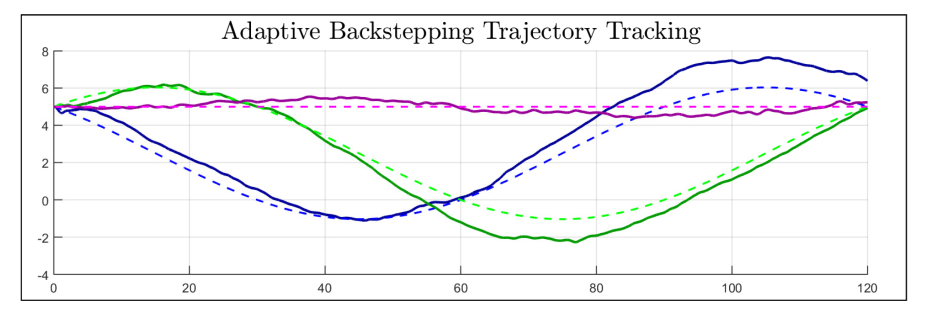
\includegraphics[width=0.8\textwidth]{graphs/ABC_Position_Trajectory}
\vspace{-12pt}
\caption{Adaptive backstepping position trajectory tracking}
\label{fig:ABC_Position_Trajectory}
\vspace{-16pt}
\end{figure}
%====================================================
\section{Allocation Tests}
\label{sec:simulation.allocator}
%====================================================
The various allocation rules, as derived in Ch:\ref{ch:allocation}, implement virtual control inputs to solve for explicit actuator positions. Each of the allocators tested here were compared with basic position and attitude Proportional Derivative controllers commanded a virtual input. 
\par
The abstraction applied to achieve an affine relationship required for inversion allocation (in Eq:\ref{eq:allocator-test}) meant that actuator transfer rates were independent from the allocation rule applied.
\begin{subequations}\label{eq:allocator-test}
\begin{equation}\label{eq:allocator-test.a}
\vec{\nu}_c=B'(\vec{\mathbf{x}},t)u=\begin{bmatrix}
\mathbb{I}_{3\times 3} & \mathbb{I}_{3\times 3} & \mathbb{I}_{3\times 3} & \mathbb{I}_{3\times 3}\\
[\vec{L}_1]_\times & [\vec{L}_2]_\times & [\vec{L}_3]_\times & [\vec{L}_4]_\times
\end{bmatrix}
\begin{bmatrix}
\vec{T}_1&
\ldots&
\vec{T}_4
\end{bmatrix}^T
\end{equation}
\vspace{-10pt}
\begin{equation}
u\cdot i = \begin{bmatrix}
\Omega_i & \lambda_i & \alpha_i
\end{bmatrix}^T = R^\dagger(\vec{\mathbf{x}},\vec{T}_i,t)~~\text{for}~i\in[1:4]
\end{equation}
\end{subequations}
The transfer rate at which physically commanded inputs implement virtually designed control inputs, $\vec{\nu}_c\rightarrow\vec{\nu}_d$, is affected by the thrust version equation $R^\dagger(\vec{\mathbf{x}},t)$, not allocation rules $B'(\vec{\mathbf{x}},t)$. The consequence of this is that, in the context of actuator transfer rates, each allocation rule performed almost identically. Inverse solutions to Eq:\ref{eq:allocation-quadratic} solve for the quadratic least squares minimized actuator positions. That means that each $|\vec{T}_i|$  within the $\mathbb{R}^{1\times 12}$ matrix $|\vec{T}_{1\rightarrow 4}|$ is minimized. The solution is an actuator cost efficient one. In general psuedo inversion, wieghted and priority normalized inverse allocators each stem from Eq:\ref{eq:inversion}: 
\begin{subequations}
\begin{equation}
\underset{u\in\mathbb{U}}{\begin{bmatrix}
\vec{T}_{1\rightarrow 4}
\end{bmatrix}}
=\big(\mathbb{I}_{m\times m}-CB(\vec{\mathbf{x}},t)\big)\vec{T}_p+C\vec{\nu}_d
\end{equation}
\vspace{-10pt}
\begin{equation}\label{eq:allocation-inversion-eq}
C=W^{-1}B^T(\vec{\mathbf{x}},t)\big(B(\vec{\mathbf{x}},t)W^{-1}B^T(\vec{\mathbf{x}},t)\big)^{-1}
\end{equation}
\end{subequations}
A combined step of setpoints for attitude \emph{and} position is used to compare each allocation rule. A pseudo inversion allocator, Eq:\ref{eq:pseudo-inversion}, is used as the reference case to which subsequent allocator algorithms are evaluated against. The typical setpoint used for both position and attitude steps, with attitude in Euler angles $\vec{\eta}_d$ not quaternions $Q_d$, is:
\begin{equation}\label{eq:simulation-state-step}
\vec{\mathbf{x}}_d=\begin{bmatrix}
\vec{\mathcal{E}}_d\\
\vec{\eta}_d
\end{bmatrix}
=
\begin{bmatrix}
\begin{bmatrix}
7.5 & 4 & 3
\end{bmatrix}^T\\
\begin{bmatrix}
-142 & 167 & -45
\end{bmatrix}^T
\end{bmatrix}~~~~\begin{bmatrix}
[\text{m}]\\
[\text{\textdegree}]
\end{bmatrix}
\end{equation}
A pseudo inversion allocation solves for $\vec{T}_{1\rightarrow 4}$ using $B^\ddagger(\vec{\mathbf{x}},t)\vec{\nu}_d$, from Eq:\ref{eq:pseudo-inversion}. Fig:\ref{fig:pseudo-inverse-step} shows the combined position and attitude step responses. The combined attitude and position step response with a pseudo inverse allocator $B^\ddagger(\vec{\mathbf{x}},t)$ settles for \emph{both} plants in $t_{95}=5.6233~[\text{s}]$ from the state step. 
\begin{figure}[hbtp]
\vspace{-12pt}
\centering
\begin{subfigure}{\textwidth}
\centering
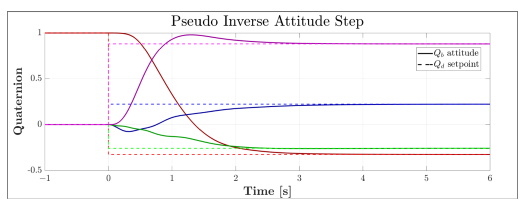
\includegraphics[width=0.8\textwidth]{graphs/pseudo_inverse_attitude}
\vspace{-12pt}
\caption{Attitude Step}
\label{fig:pseudo_inverse_attitude}
\end{subfigure}
\begin{subfigure}{\textwidth}
\vspace{-3pt}
\centering
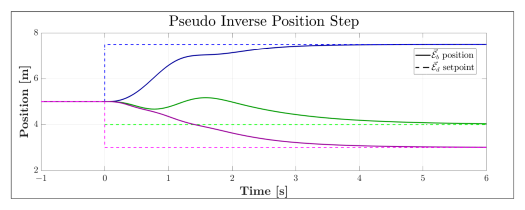
\includegraphics[width=0.8\textwidth]{graphs/pseudo_inverse_position}
\vspace{-12pt}
\caption{Position Step}
\label{fig:pseudo_inverse_position}
\end{subfigure}
\vspace{-8pt}
\caption{Pseudo-Inverse step response}
\label{fig:pseudo-inverse-step}
\vspace{-24pt}
\end{figure}
\par
The preferred allocator positions, described in Sec:\ref{subsec:allocation.allocators.norminverse}, are hovering conditions defined with respect to either the inertial or body frames, $\mathcal{F}^{I}$ and $\mathcal{F}^{b}$. At steady state with an attitude at the origin, $Q_d=[1~\vec{0}]^T$; the controller commands the virtual control input:
\begin{equation}\label{eq:hover-actuator}
\vec{\nu}_p=\begin{bmatrix}
\vec{F}_p\\
\vec{\tau}_p
\end{bmatrix}
=
\begin{bmatrix}
\begin{bmatrix}
0&0&15.45
\end{bmatrix}^T
\\
\begin{bmatrix}
0.25&
0.50&
-1.89
\end{bmatrix}^T
\end{bmatrix}~~~~\begin{bmatrix}
[\text{N}]\\
[\text{N.mm}]
\end{bmatrix}^T~~~~\in\mathcal{F}^{b,I}
\end{equation}
The small amount of control torque applied in Eq:\ref{eq:hover-actuator}, about the $\hat{Z}_{I/b}$ axis, is to compensate for net gravitational torque due to the eccentric center of gravity and resultant aerodynamic torque $\vec{\tau}_Q$ from the propellers rotational velocity. Applying the pseudo inverse allocation rule to the preferred input $\vec{\nu}_p$ gives the following actuator positions which effect hovering conditions:
\begin{subequations}\label{eq:preffered-hover-inertia}
\begin{equation}
\vec{T}_p^{I}=B^\ddagger(\mathbf{x},t)\vec{\nu}_p=\begin{bmatrix}
T_{1x}&T_{1Y}&T_{1Z}&\ldots~\ldots&T_{4x}&T_{4y}&T_{4z}
\end{bmatrix}
\end{equation}
\vspace{-24pt}
\begin{equation}
=\begin{bmatrix}
\begin{bmatrix}
0.00 & -0.02 & 3.86
\end{bmatrix} 
&
\begin{bmatrix}
0.02 & 0 & 3.86
\end{bmatrix}
&
\begin{bmatrix}
0 & 0.02 & 3.86
\end{bmatrix}
&
\begin{bmatrix}
-0.02 & 0 & 3.86
\end{bmatrix}
\end{bmatrix}^T~~~~[\text{N}]
\end{equation}
\end{subequations}
Testing the same attitude and position setpoint steps, but with preferred actuator hovering conditions relative to the inertial frame (illustrated in Fig:\ref{fig:hover-inertial}) produces a response shown in Fig:\ref{fig:inertial-norm-step}. The plant settles in $t_{95}=5.617~[\text{s}]$ with a practically identical response to the pseudo-inverse case presented before in Fig:\ref{fig:pseudo-inverse-step}.
\begin{figure}[hbtp]
\vspace{-12pt}
\centering
\begin{subfigure}{\textwidth}
\centering
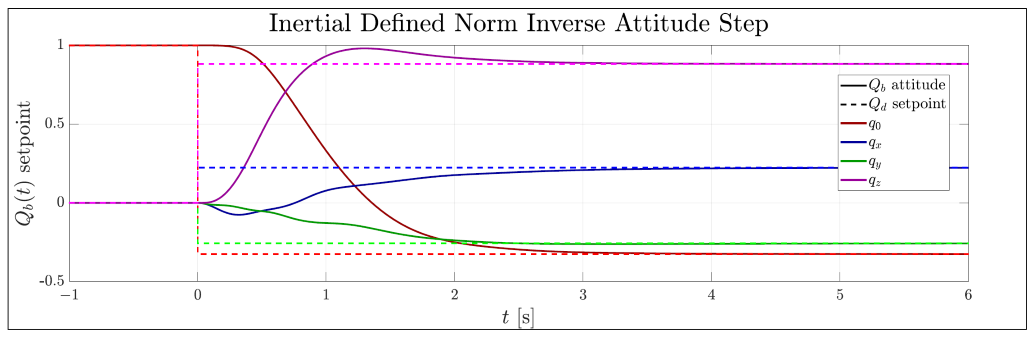
\includegraphics[width=0.8\textwidth]{graphs/inertial_norm_attitude}
\vspace{-12pt}
\caption{Attitude Step}
\label{fig:inertial_norm_attitude}
\end{subfigure}
\begin{subfigure}{\textwidth}
\vspace{-2pt}
\centering
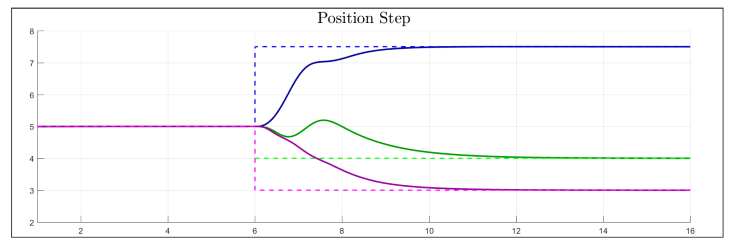
\includegraphics[width=0.8\textwidth]{graphs/inertial_norm_position}
\vspace{-6pt}
\caption{Position Step}
\label{fig:inertia_norm_position}
\vspace{-8pt}
\end{subfigure}
\caption{Inertial hover preferred actuator step response}
\label{fig:inertial-norm-step}
\vspace{-18pt}
\end{figure}
\par
Transformation of those hovering conditions in Eq:\ref{eq:hover-actuator} from the inertial frame to the body frame is applied through an instantaneous quaternion transformation:
\begin{equation}
\vec{\nu}_p\text{}\hspace{-2pt}'=\begin{bmatrix}
Q_b\otimes\vec{F}_p\otimes Q_b^*\\
Q_b\otimes\vec{\tau}_p\otimes Q_b^*
\end{bmatrix}~~~~\in\mathcal{F}^{b}
\end{equation}
The hovering conditions are then always a function of the body's instantaneous attitude. However, because the control plant only tracks first order setpoints the control plant's response then always tends towards stability at each controller interval. As a result the control law always aims at tending towards hovering conditions, irrespective of the allocator rule applied. Again the plant settles in roughly the same time, $t_{95}=5.614~[\text{s}]$, with a response shown in Fig:\ref{fig:body-norm-step}.
\par
\begin{figure}[hbtp]
\centering
\begin{subfigure}{\textwidth}
\centering
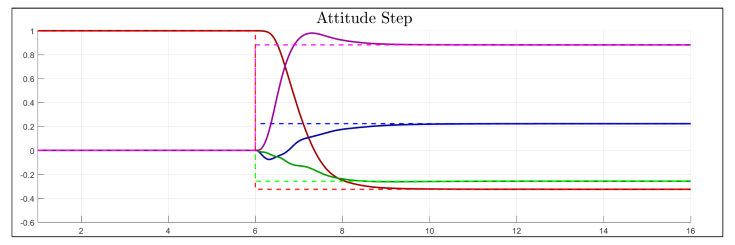
\includegraphics[width=0.8\textwidth]{graphs/body_norm_attitude}
\vspace{-12pt}
\caption{Attitude Step}
\label{fig:body_norm_attitude}
\end{subfigure}
\begin{subfigure}{\textwidth}
\vspace{-3pt}
\centering
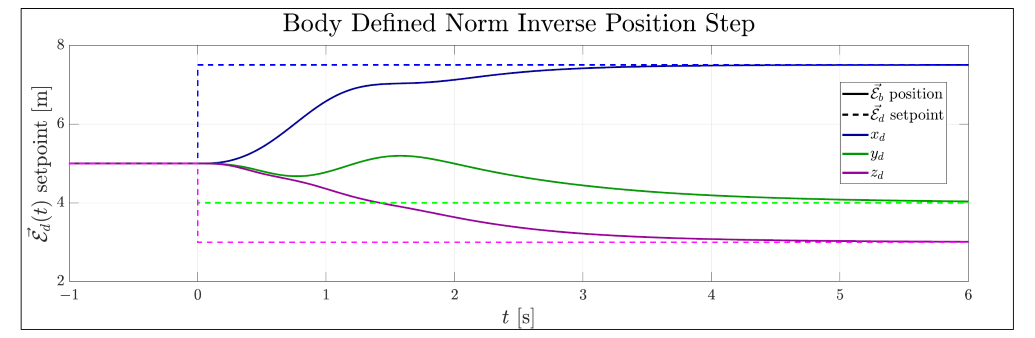
\includegraphics[width=0.8\textwidth]{graphs/body_norm_position}
\vspace{-12pt}
\caption{Position Step}
\label{fig:body_norm_position}
\end{subfigure}
\vspace{-8pt}
\caption{Body frame hover preferred actuator step response}
\label{fig:body-norm-step}
\vspace{-16pt}
\end{figure}
\par
The weighted actuator allocation rule, proposed in Sec:\ref{subsec:allocation.allocators.weightedinverse}, prioritizes the use of different input thrust components in Eq:\ref{eq:allocator-test.a}. The weighting matrix is a $12\times 12$ set of coefficients which bias various allocators as illustrated in Fig:\ref{fig:weighted-matrix}. In order to reduce slack and ensure setpoint tracking , being the primary control objective, each weighting coefficient row and column was constrained to a normalized summation. Furthermore it was proposed that coefficients were selected based on an optimization as per the penalty function Eq:\ref{eq:actuator-penalty}. In practice the weighting coefficients have no bearing on the input plant settling time for each actuator module; to demonstrate a weighted actuator case the following weighting matrix was used for $C=W^{-1}B^T(B.W^{-1}.B^T)^{-1}$ from Eq:\ref{eq:allocation-inversion-eq}:
\begin{equation}\label{eq:inversion-weights}
W\triangleq
\begin{bmatrix}
\begin{bmatrix}
72 & 9 & 9\\
9 & 72 & 9\\
9 & 9 & 72
\end{bmatrix}
&
\begin{bmatrix}
0 & 0 & 0\\
0 & 0 & 0\\
0 & 0 & 0
\end{bmatrix}
&
\begin{bmatrix}
8 & 1 & 1\\
1 & 8 & 1\\
1 & 1 & 8
\end{bmatrix}
&
\begin{bmatrix}
0 & 0 & 0\\
0 & 0 & 0\\
0 & 0 & 0
\end{bmatrix}
\\
\begin{bmatrix}
0 & 0 & 0\\
0 & 0 & 0\\
0 & 0 & 0
\end{bmatrix}
&
\begin{bmatrix}
72 & 9 & 9\\
9 & 72 & 9\\
9 & 9 & 72
\end{bmatrix}
&
\begin{bmatrix}
0 & 0 & 0\\
0 & 0 & 0\\
0 & 0 & 0
\end{bmatrix}
&
\begin{bmatrix}
8 & 1 & 1\\
1 & 8 & 1\\
1 & 1 & 8
\end{bmatrix}
\\
\begin{bmatrix}
8 & 1 & 1\\
1 & 8 & 1\\
1 & 1 & 8
\end{bmatrix}
&
\begin{bmatrix}
0 & 0 & 0\\
0 & 0 & 0\\
0 & 0 & 0
\end{bmatrix}
&
\begin{bmatrix}
72 & 9 & 9\\
9 & 72 & 9\\
9 & 9 & 72
\end{bmatrix}
&
\begin{bmatrix}
0 & 0 & 0\\
0 & 0 & 0\\
0 & 0 & 0
\end{bmatrix}
\\
\begin{bmatrix}
0 & 0 & 0\\
0 & 0 & 0\\
0 & 0 & 0
\end{bmatrix}
&
\begin{bmatrix}
8 & 1 & 1\\
1 & 8 & 1\\
1 & 1 & 8
\end{bmatrix}
&
\begin{bmatrix}
0 & 0 & 0\\
0 & 0 & 0\\
0 & 0 & 0
\end{bmatrix}
&
\begin{bmatrix}
72 & 9 & 9\\
9 & 72 & 9\\
9 & 9 & 72
\end{bmatrix}
\end{bmatrix}\times 10^{-3}
\end{equation}
The weighted allocator's response in Fig:\ref{fig:weighted-inverse-step} shows the minor differences between each of the above allocation rules. The final weighted inversion allocator applied with Eq:\ref{eq:inversion-weights} settled in $t_{95}=5.618$. The inversion based allocator's requirement for an affine effectiveness relationship meant that actuator transfer functions were separated from the allocation block, this made the actuator transfer rates independent from the allocation rule applied. Because of the requirements that each allocator still meets the slack variable requirements of setpoint tracking, each allocator's performance is much of the same. The 12 produced thrust component inputs are, within a margin of error, effectively the same across each allocation rule\ldots
\newpage
\begin{figure}[hbtp]
\centering
\begin{subfigure}{\textwidth}
\centering
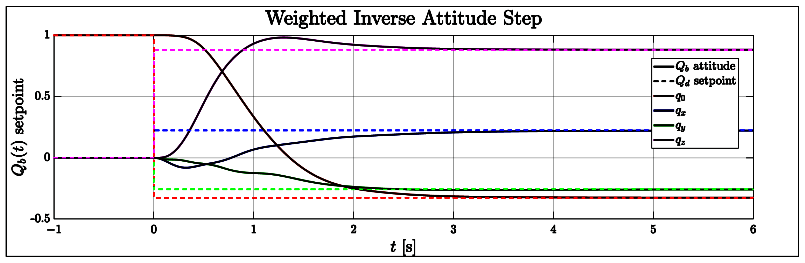
\includegraphics[width=0.8\textwidth]{graphs/weighted_inverse_attitude}
\vspace{-10pt}
\caption{Attitude Step}
\label{fig:weighted_inverse_attitude}
\end{subfigure}
\begin{subfigure}{\textwidth}
\vspace{-3pt}
\centering
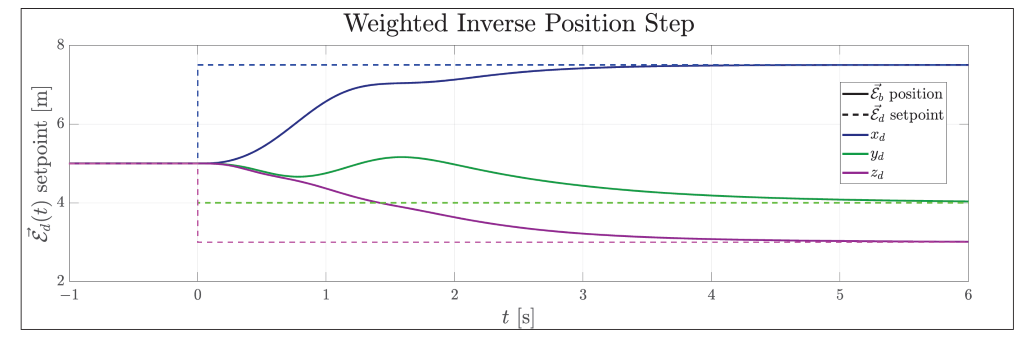
\includegraphics[width=0.8\textwidth]{graphs/weighted_inverse_position}
\vspace{-10pt}
\caption{Position Step}
\label{fig:weighted_inverse_position}
\end{subfigure}
\vspace{-8pt}
\caption{Weighted actuator allocation step response}
\label{fig:weighted-inverse-step}
\vspace{-16pt}
\end{figure}
%====================================================
\section{Input Saturation}
\label{sec:simulation.saturation}
%====================================================
The introduction of a rotational limit to the actuating servos was a design decision made previously in Sec:\ref{subsec:proto.design.transfer}. The $\pm 90\text{\textdegree}$ limit on the servos is something which can easily be solved by changing the mechanical design to incorporate continuous rotation actuators. The standard state setpoint step used thus far \emph{do not} command any of the actuators beyond their rotational limits, neither does the applied trajectory tracking loop. Alternatively, the following state setpoint is used:
\begin{equation}\label{eq:saturation-state-step}
\vec{\mathbf{x}}_d\text{}\hspace{-2pt}'=
\begin{bmatrix}
\vec{\mathcal{E}}_d\text{}\hspace{-2pt}'\\
\vec{\eta}_d\text{}\hspace{-2pt}'
\end{bmatrix}
=\begin{bmatrix}
\begin{bmatrix}
7.5 & 4 & 3
\end{bmatrix}^T
\\
\begin{bmatrix}
-142 & 35 & -45
\end{bmatrix}^T
\end{bmatrix}
~~~~\begin{bmatrix}
[\text{m}]\\
[\text{\textdegree}]
\end{bmatrix}
\end{equation}
The attitude setpoint, $\vec{\eta}_d\text{}\hspace{-2pt}'$, was chosen because it commands each servo beyond their rotational limit. When using Proprotional Derivative controllers for both position and attitude control loops, Fig:\ref{fig:unsaturated-step} shows that step response for attitude and positions collectively.
\begin{figure}[hbtp]
\vspace{-4pt}
\centering
\begin{subfigure}{\textwidth}
\centering
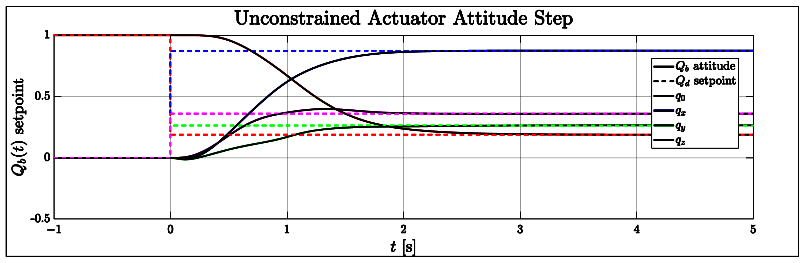
\includegraphics[width=0.8\textwidth]{graphs/unsaturated-attitude-step}
\vspace{-6pt}
\caption{Attitude step}
\label{fig:unsaturated-attitude-step}
\end{subfigure}
\vspace{-18pt}
\end{figure}
\newpage
\begin{figure}[htbp]
\vspace{-12pt}
\centering
\begin{subfigure}{\textwidth}
\centering
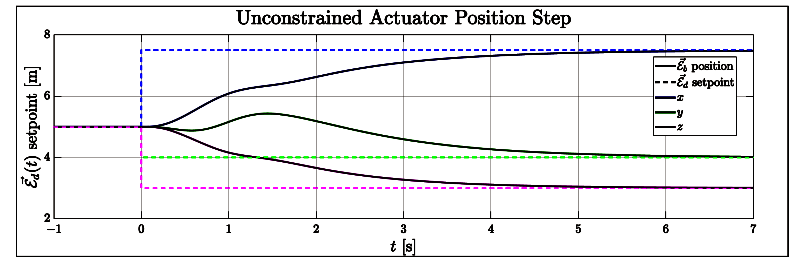
\includegraphics[width=0.8\textwidth]{graphs/unsaturated-position-step}
\vspace{-8pt}
\caption{Position step}
\label{fig:unsaturated-position-step}
\end{subfigure}
\vspace{-10pt}
\caption{Step response without servo limits}
\label{fig:unsaturated-step}
\vspace{-10pt}
\end{figure}
\par
Neither responses in Fig:\ref{fig:unsaturated-step} are anything unexpected. The rotational positions for all eight servos are shown in Fig:\ref{fig:unsaturated-servos}. Noting that each middle ring servo, $\alpha_i$, settles to both above and below the $\pi/2$ rotational limit.
\begin{figure}[hbtp]
\vspace{-12pt}
\centering
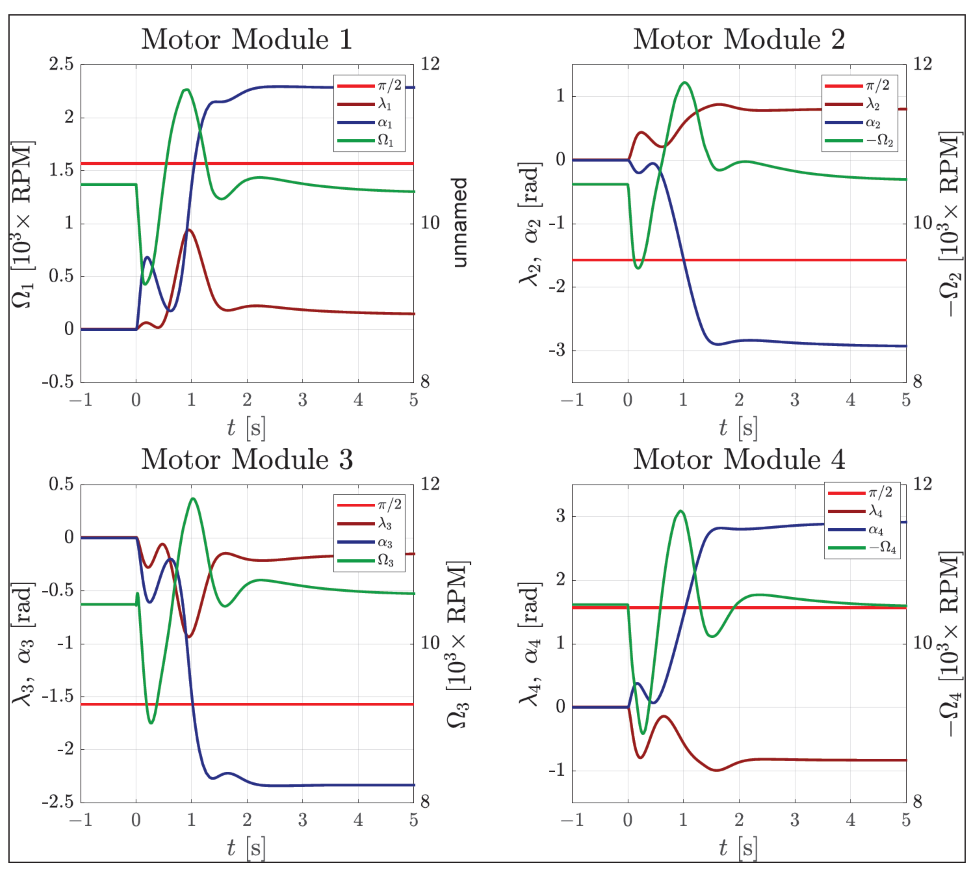
\includegraphics[width=0.67\textwidth]{graphs/unsaturated-servos}
\vspace{-12pt}
\caption{Servo inputs without limits}
\label{fig:unsaturated-servos}
\vspace{-20pt}
\end{figure}
\par
Then introducing that hard limit to the state step in Eq:\ref{eq:saturation-state-step} produces a step response in Fig:\ref{}. The response obviously never reaches a settling point and destabilizes when the actuator saturation limits are applied.
\begin{figure}[hbtp]
\vspace{-12pt}
\centering
\begin{subfigure}{\textwidth}
\centering
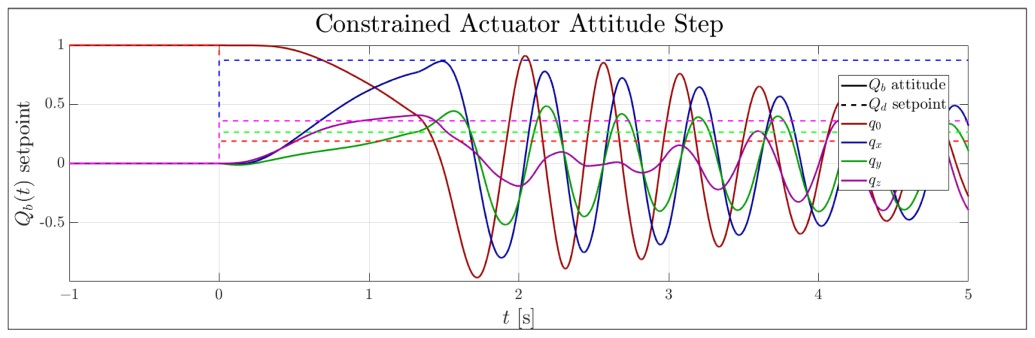
\includegraphics[width=0.8\textwidth]{graphs/saturated-attitude-step}
\vspace{-10pt}
\caption{Attitude step}
\vspace{-16pt}
\end{subfigure}
\vspace{-24pt}
\end{figure}
\newpage
\begin{figure}\ContinuedFloat
\vspace{-8pt}
\centering
\begin{subfigure}{\textwidth}
\centering
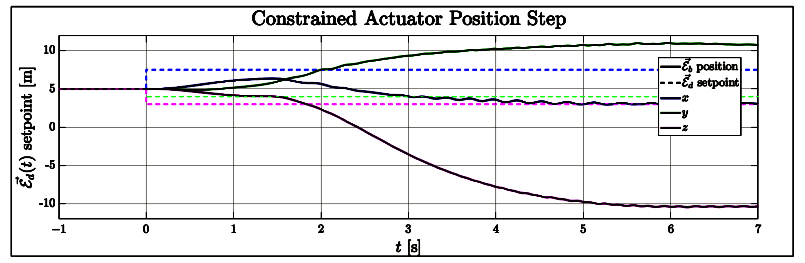
\includegraphics[width=0.8\textwidth]{graphs/saturated-position-step}
\vspace{-10pt}
\caption{Position step}
\end{subfigure}
\vspace{-6pt}
\caption{Step response with servo limits}
\vspace{-18pt}
\end{figure}
\par
Fig:\ref{fig:saturated-servos} shows the limit cycles which the servos get stuck in when an attitude step which exceeds their hard limit is commanded.
\begin{figure}[hbtp]
\vspace{-8pt}
\centering
\includegraphics[width=0.67\textwidth]{graphs/saturated-servos}
\vspace{-6pt}
\caption{Servo inputs without limits}
\label{fig:saturated-servos}
\end{figure}
%====================================================
\section{State Estimation}
\label{sec:simulation.state}
%====================================================
The final aspect of the control simulation to test is the effect state estimation will have on the setpoint tracking. It was proposed, in Ch:\ref{ch:proto}, that a 9-axis inertial measurement unit would produce inertial rates in the body frame. Then some form of filtration would fuse sensor measurements together to provide state estimation for the attitude. It is difficult to approximate position displacement in the inertial frame with only an IMU, that is why it was proposed that a motion camera VICON-like system, \cite{arnold} would track the vehicles position under testing conditions. 
\par
Such components of the control loop could indeed be constructed in simulation but, owing to the large amounts of noise a physical flight test would induce, would not prove useful in evaluating the efficacy of the net proposed control system. Given the amount of vibrations and disturbances the prototype will undergo, simulations won't be able to accurately approximate such affects. Instead it was deemed pertinent to only apply discretization effects onto the state feedback elements within the control loop.
\par
Quaternion position, angular velocity and translational velocity signals were discretized and sampled at a rate of $70~[Hz]$ to emulate an IMU system based on the hardware proposed (Sec:\ref{sec:proto.layout}). In reality those signals would be processed by a Kalman filter and be subject to a relative degree of noise and integral drift. Then inertial position feedback was sampled at $50~[\text{Hz}]$ to emulate the proposed camera system \cite{arnold}.
\par
Both position and attitude control loops, testing with the basic Proportional Derivative controllers in both cases, were stable for the above proposed sampling rates. In fact the entire system was stable for sample rates as slow as $5~[\text{Hz}]$, whose response for a typical attitude and position step (Eq:\ref{eq:simulation-state-step}) is plotted in Fig:\ref{fig:discrete_step}.
\begin{figure}[hbtp]
\centering
\begin{subfigure}{\textwidth}
\centering
\includegraphics[width=0.8\textwidth]{graphs/discrete_attitude_step}
\vspace{-12pt}
\caption{Attitude step}
\end{subfigure}
\begin{subfigure}{\textwidth}
\vspace{-3pt}
\centering
\includegraphics[width=0.8\textwidth]{graphs/discrete_position_step}
\vspace{-12pt}
\caption{Position step}
\end{subfigure}
\vspace{-8pt}
\caption{Discretized state steps}
\label{fig:discrete_step}
\vspace{-12pt}
\end{figure}
\par
Fig:\ref{fig:feasible-attitude} shows the range of feasible attitude setpoints achievable by the control loop when the actuator rotational limit is applied.
\begin{figure}[htbp]
\centering
\includegraphics[width=0.4\textwidth]{figs/feasible-attitude}
\caption{Feasible attitude setpoints}
\label{fig:feasible-attitude}
\end{figure}